\documentclass[10pt]{article}
\usepackage[scale=0.80]{geometry}
%\usepackage{graphicx}  % Required for including pictures
\usepackage[pdftex]{graphicx}
\usepackage{float} % Allows putting an [H] in \begin{figure} to specify the exact location of the figure
\usepackage{wrapfig} % Allows in-line images
\usepackage[british,UKenglish,USenglish,english,american]{babel}
%\usepackage[utf8]{inputenc} %T1 ou utf8 latin1
\usepackage{ragged2e}
\usepackage{amsmath}
\usepackage{array}
\usepackage{multirow}
\usepackage{color}
\usepackage{float}
\definecolor{gray}{gray}{0.20} %pourcentage de gris
\definecolor{red2}{cmyk}{0,1,0.99,0.04}	% cyan, magenta, jaune et noir

\title{\begin{Large}
\textbf{Benchmark test : Fetch-limited growth}\\
\end{Large}}
\author{Marine Le Gal - Elodie Gagnaire Renou - Michel Benoit}
\begin{document}
\maketitle 

\section{Purpose}
The goal of this test-case is to validate the generation (Source/sink terms)  and the growth of the wave spectrum depending of the length of wind action (fetch) with a constant wind defined at 10 meters from the sea surface. The domain used is simple and we want to observe the evolution of few parameters along its length, as the significant wave height, peak period and variance spectrum. 
It is supposed that the wind blew long enought to have reached a steady state.\\
Thus, this benchmark will allow us to compare and validate the different models of wind generation (three models), whitecapping dissipation (two models), non-linear quadruplet interactions (three models but only two are used here). Friction bottom dissipation and eventually depth-induced breaking dissipation (four models) is also included when a finite depth is imposed. The models used are presented in the table 1.\\ \quad \\
\vspace{1cm}
\hspace{-2cm}
\begin{table}
\hspace{-1.54cm}
\begin{tabular}{|c|c|c|c|c|c|c|c|}
\hline
Models & Wind generation  & white capping  & Quadruplet  & Depth & Bottom friction & Depth-induced breaking \\
 &  model &  model &  transfers formula &  &  coeff. &  dissipation model\\\hline
test 1 & Janssen & Komen et al. (1984);& DIA* & $\inf$ & -- & --\\
 &  (1989);(1991) & Janssen et al.  ;(1991)  & &  &  & \\
\hline
test 2  & Snyder (1981) & Komen et al. ;  & DIA & $\inf$ & --& --\\
 &  & Janssen et al. & &  & &\\
\hline
test 3 & Snyder & Westhuysen et al(2007) & DIA & $\inf$ & --& -- \\
\hline
test 4 & Yan (1987) & Westhuysen & DIA & $\inf$ & --& -- \\
\hline
test 5 & Snyder & Westhuysen et al& Exact GQM**  & $\inf$ & --& --\\
 &  &  &  coarse discretization & & & \\ \hline
 test 6 & Janssen &Komen et al. ;  & Exact GQM  & $\inf$ & -- & --\\
 &  & Janssen et al.  &  coarse discretization & & & \\ \hline
 test 6b & Janssen & Komen et al. ;& Exact GQM & $\inf$ & -- & --\\
  &  & Janssen et al.   &  medium discretization & & & \\ \hline\hline
test 7a & Snyder & Westhuysen et al& DIA & 180 & 0.038 & -- \\
 test 7b & Snyder & Westhuysen et al& DIA & 60 & 0.038& -- \\
 test 7c & Snyder & Westhuysen et al& DIA & 30 & 0.038& -- \\
  test 7d & Snyder & Westhuysen et al& DIA & 15 & 0.038& -- \\
   test 7e & Snyder & Westhuysen et al& DIA & 5 & 0.038& Battjes \& Janssen \\ 
    &  & &  & & &(V = 20m/s) \\ \hline
 \end{tabular}
 \caption{Different models used for this test-case. In all cases, linear wave growth term from the formula of Cavaleri and
Malanotte-Rizzoli (1981) is used.\textit{* : Discrete Interaction Approximation,Hasselmann et al., 1985. ** : Gaussian Quadrature Method,introduced by Lavrenov
[Lavrenov, 2001] and implemented by Benoit and Gagnaire-Renou [Gagnaire-Renou et al., 2010]}}
\end{table}
\section{Referent experiments}
In order to validate TOMAWAC's results, they will be compared to different empirical formulas:
\begin{itemize}
\item Infinite depth :
\subitem JONSWAP (Hasselmann and al. 1973)
\subitem CERC (1977)
\subitem Wilson and Goda (1965 , 2003)
\subitem Kahma and Calkoen (1992)
\item Finite depth :
\subitem CERC (1984)
\end{itemize}
\section{Test-case description}

\subsection{Geometry of the domain and bathymetry}
\begin{tabular}{ccc}
Domain & dimension :& 1000 km * 500 km\\
 Depth constant along the domain :& test 7a & 180 m\\
 & test 7b & 60 m\\ 
& test 7c & 30 m\\ 
& test 7d & 15 m\\
& test 7e & 5 m\\
 & or infinite\\
\end{tabular}
\subsection{Mesh}
Several meshes have been tested. The important point highlighted by the analysis is at the begining of the fech the mesh must be sufficiently fine. At the end, the "free" mesh has been kept because it is the most used in industry and maritime applications (can be adapted to coast).
\quad \vspace{3cm}
\begin{figure}[H]
  \centering
    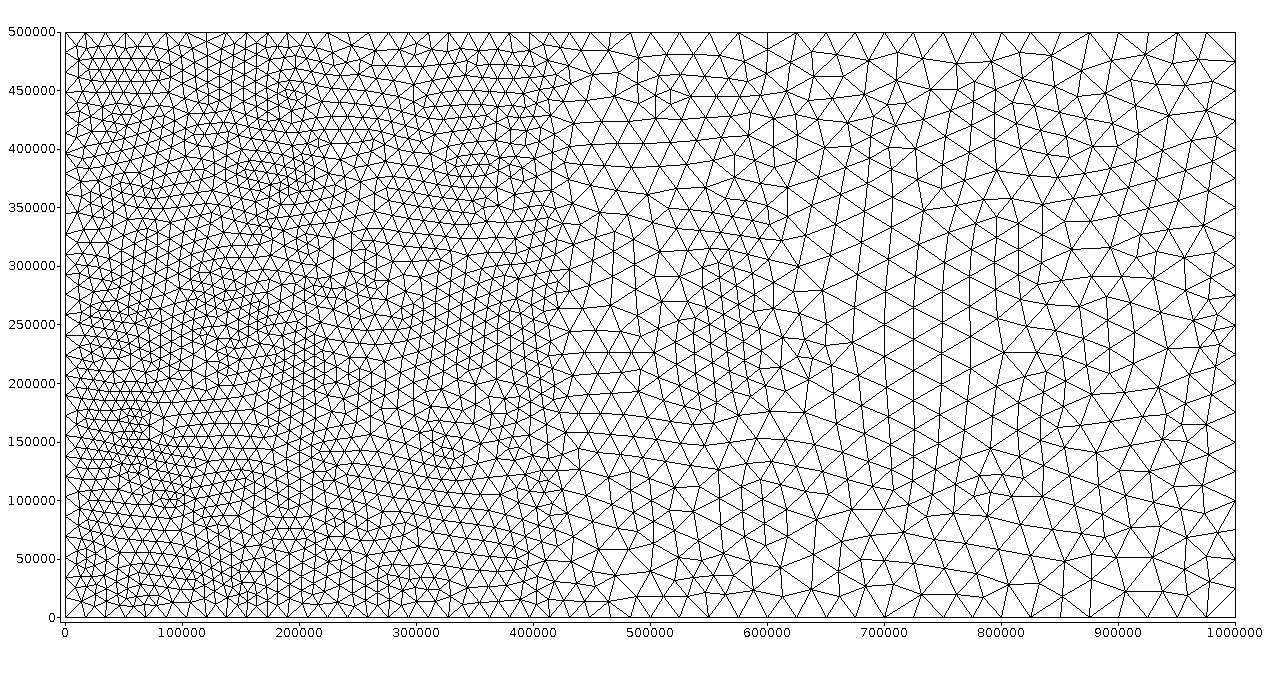
\includegraphics[scale = 0.35]{freemesh.png}
      \caption{Free and refined mesh $\Delta x_{bigger} \approx 25 000 m$ - $\Delta x_{medium} \approx 20 000 m$ - $\Delta x_{smaller} \approx 10 000 m$}
\end{figure}

\subsubsection{Spectro-angular discretization}
\begin{itemize}
\item 50 frequencies ($f_1 $= 0.04 Hz for $U_{10} = 20m/s$, $f_1 $= 0.08 Hz for $U_{10} = 10m/s$ with geometric spacing q = 1.05)
\item 36 directions uniformly distributed
\end{itemize}

\subsection{Initial and Boundary conditions}
Jonswap spectrum has been set as initial condition.\\
The domain is a part of a sea. A constant and homogeneous wind blows perpendicular to a long and straight coastline. The boundary conditions are shown in Figure 2:
\begin{figure}
\centering
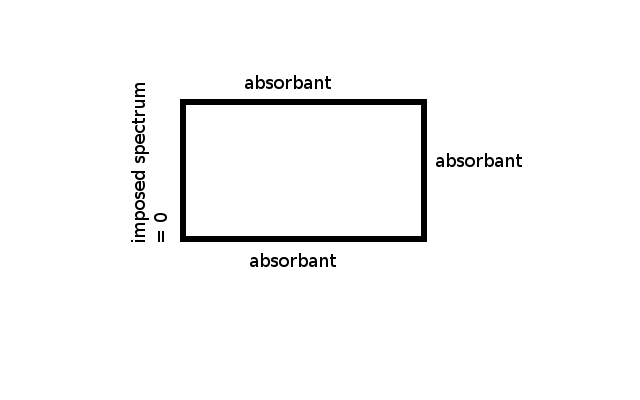
\includegraphics[scale=0.5]{boundarycond.jpg}
\caption{Boundary conditions}
\end{figure}
\section{Numerical parameters}
\begin{itemize}
\item time step : 900s
\item physical time reached : 48 h
\item caracterization of the computer : \subitem Core : Linux 2.6.32-5-amdb64 \subitem Processors : Intel(R) 
xeon(R) CPU E5620 @ 2.4Ghz
\item CPU times : \\
\begin{tabular}{c|c|c|c|c}
 & tests 1/2/3/4 & test 5/6 &tests 6b & tests 7\\
 \hline
CPU times & 3min & 3h25 & 5h40 & 25 s \\
\end{tabular}
\end{itemize}

\section{TOMAWAC Results - infinite depth }
\subsection{Wave's growth depending of the fetch for different wind velocities}
The figure 3 shows the significant wave heights and the peak periods of waves along the fetch (along the axis $ y = 250 km$ ) for the test 1 (the others are not shown because they give the same conclusions). These curves are obtained after 48 hour of wind action for a wind of 5 to 25 m/s. It is clearly seen that the wind has a considerable impact on these values and bigger waves are obtained with stronger wind. Also, stronger is the wind, longer is the fetch needed to reach the steady state. It can be noticed that the significant wave height does not grow linearly but following the squared wind velocity.
\begin{figure}[H]
  \centering
  	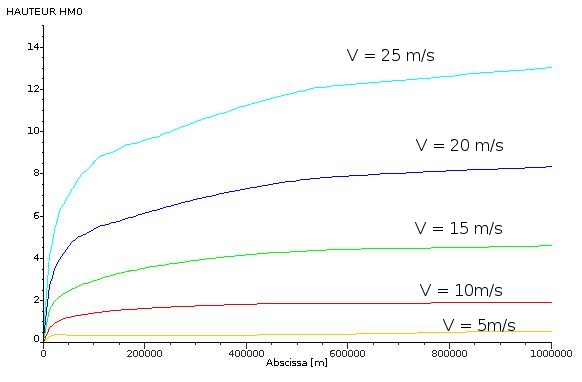
\includegraphics[width=0.5\textwidth]{Hm0_free_mesh.jpg}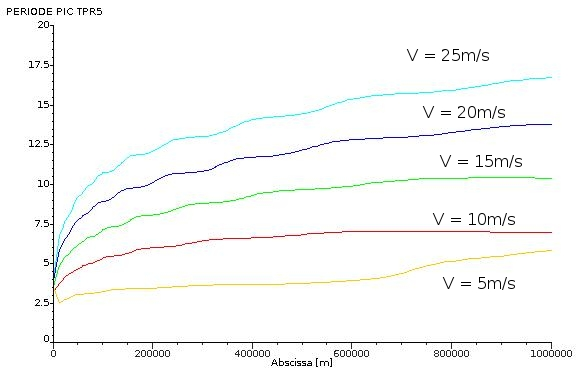
\includegraphics[width=0.5\textwidth]{Tp_free_mesh.jpg}
      \caption{Significant wave heights and peak periods for the first test, $U_{10} = 5 - 10 - 15 - 20 - 25 m/s$}
\end{figure}
\subsection{Non-dimensionnal variances and peak frequencies}
Here all the tests are compared, but only with a 20m/s and 10m/s winds. The value obtained with TOMAWAC V6P2 are compared with the empirical formulas : JONSWAP (Hasselmann and al. 1973), CERC (1977), Wilson and Goda (1965 \& 2003), Kahma and Calkoen (1992). The non-dimensionnal variables are :\\
\begin{figure}[H]
  \centering
  	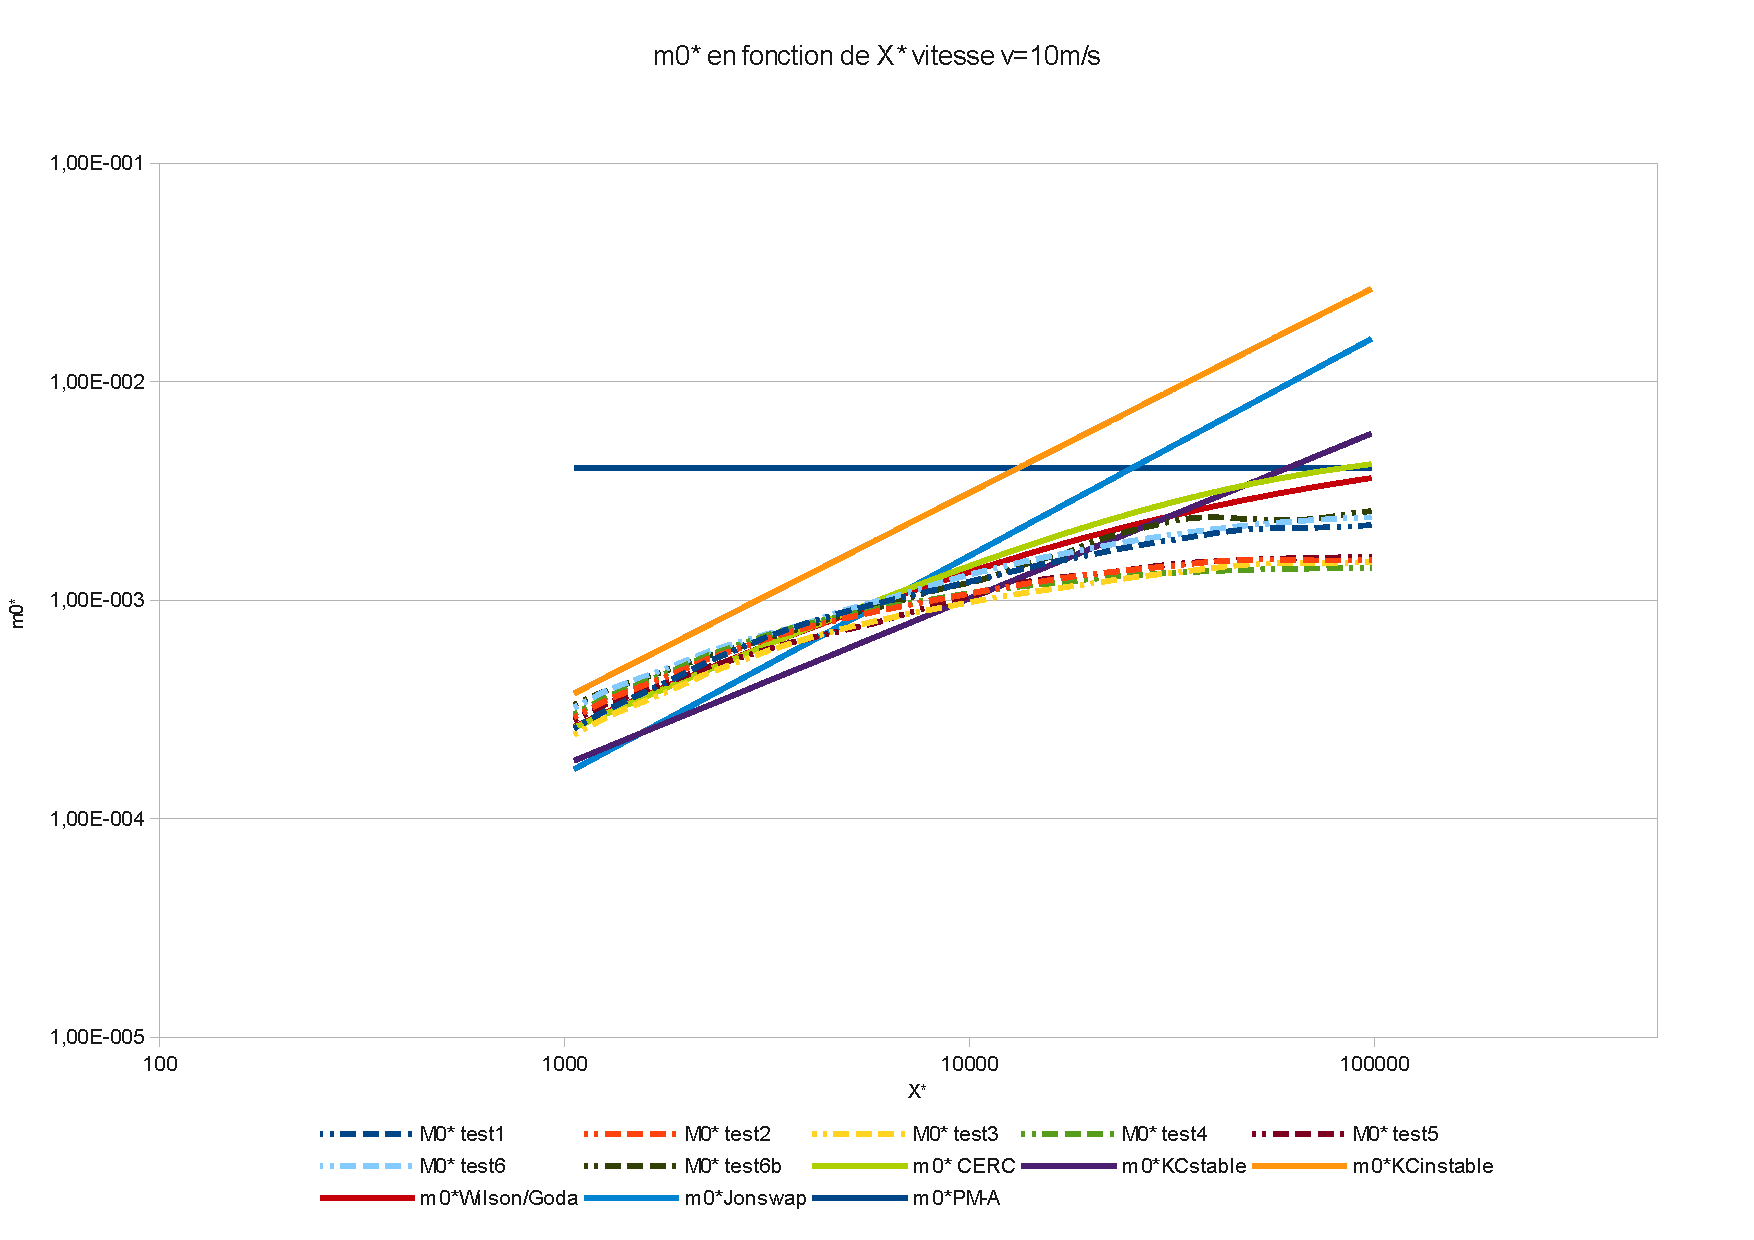
\includegraphics[width=0.5\textwidth]{M0v10id.pdf}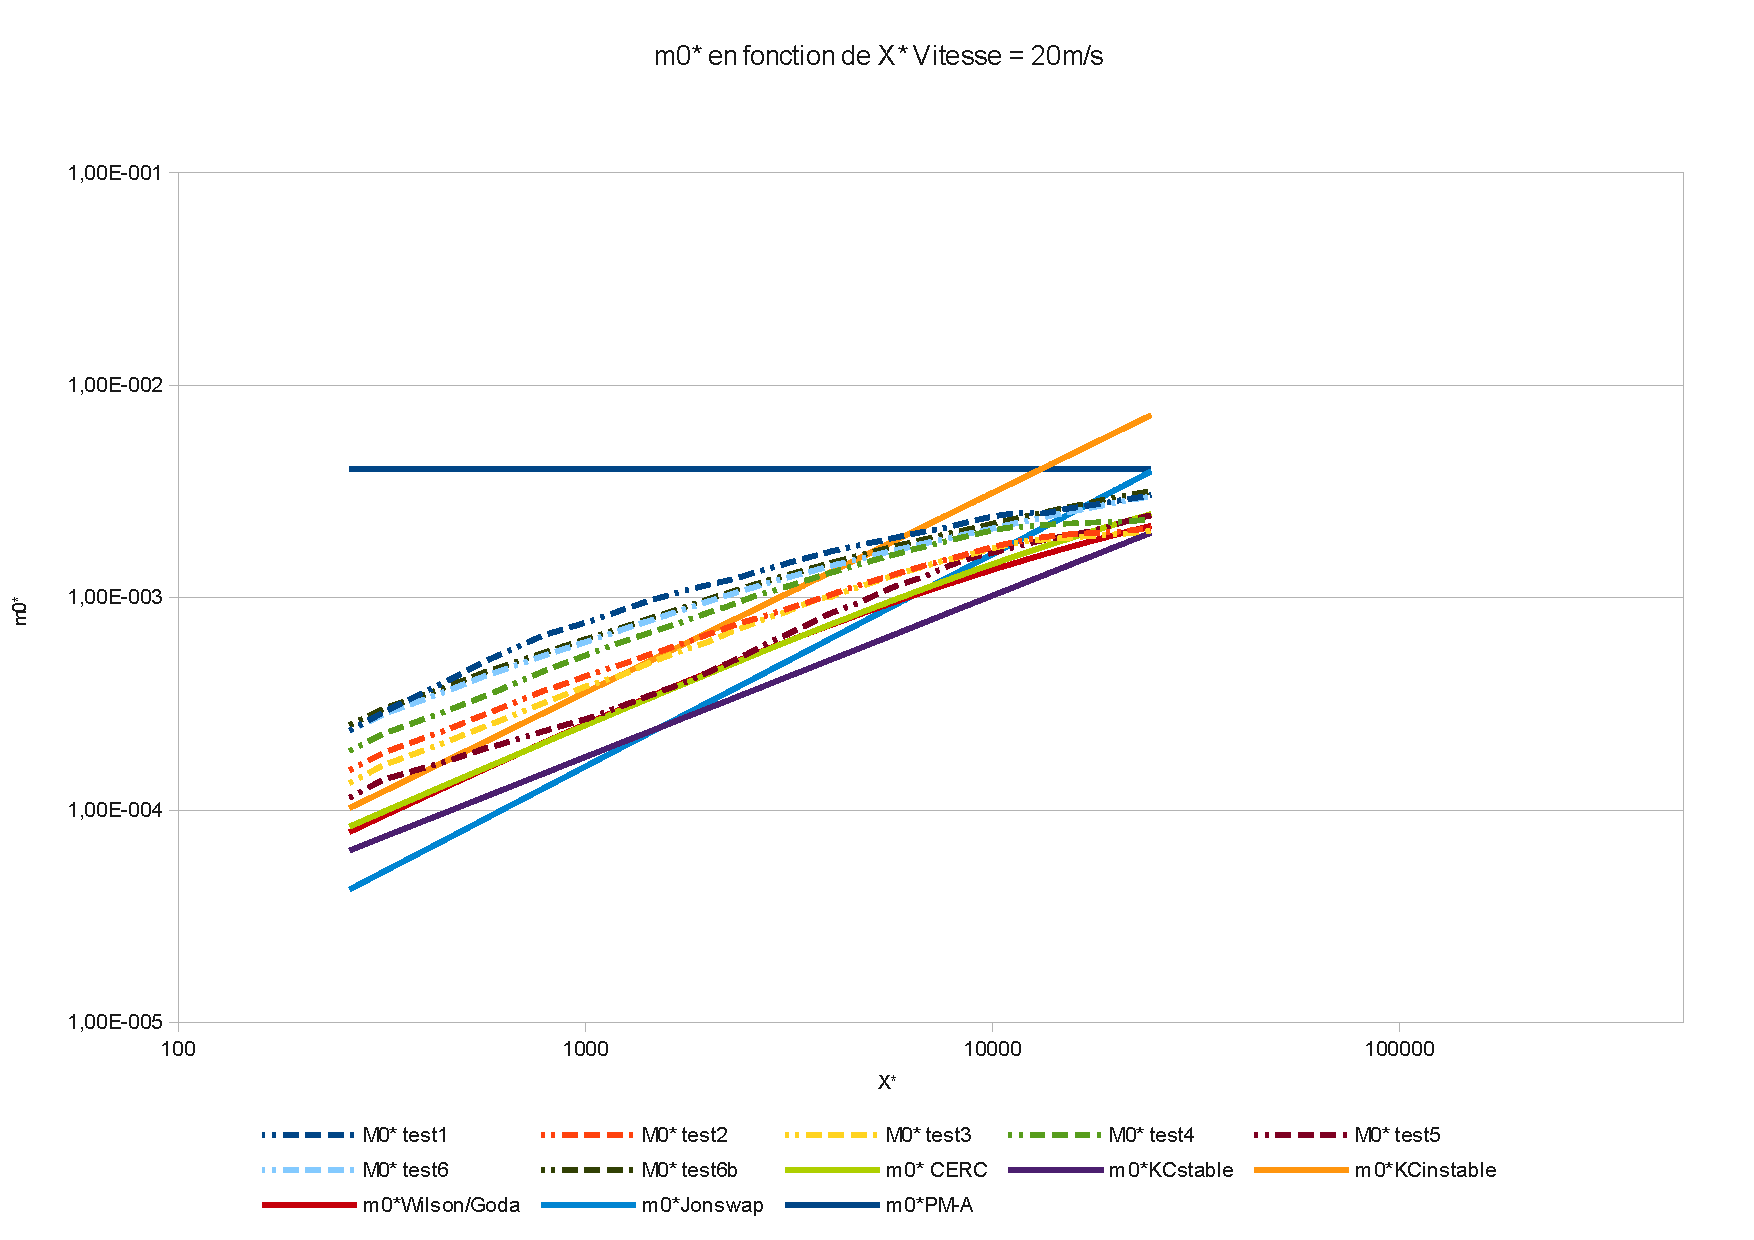
\includegraphics[width=0.5\textwidth]{M0v20id.pdf}\\
  	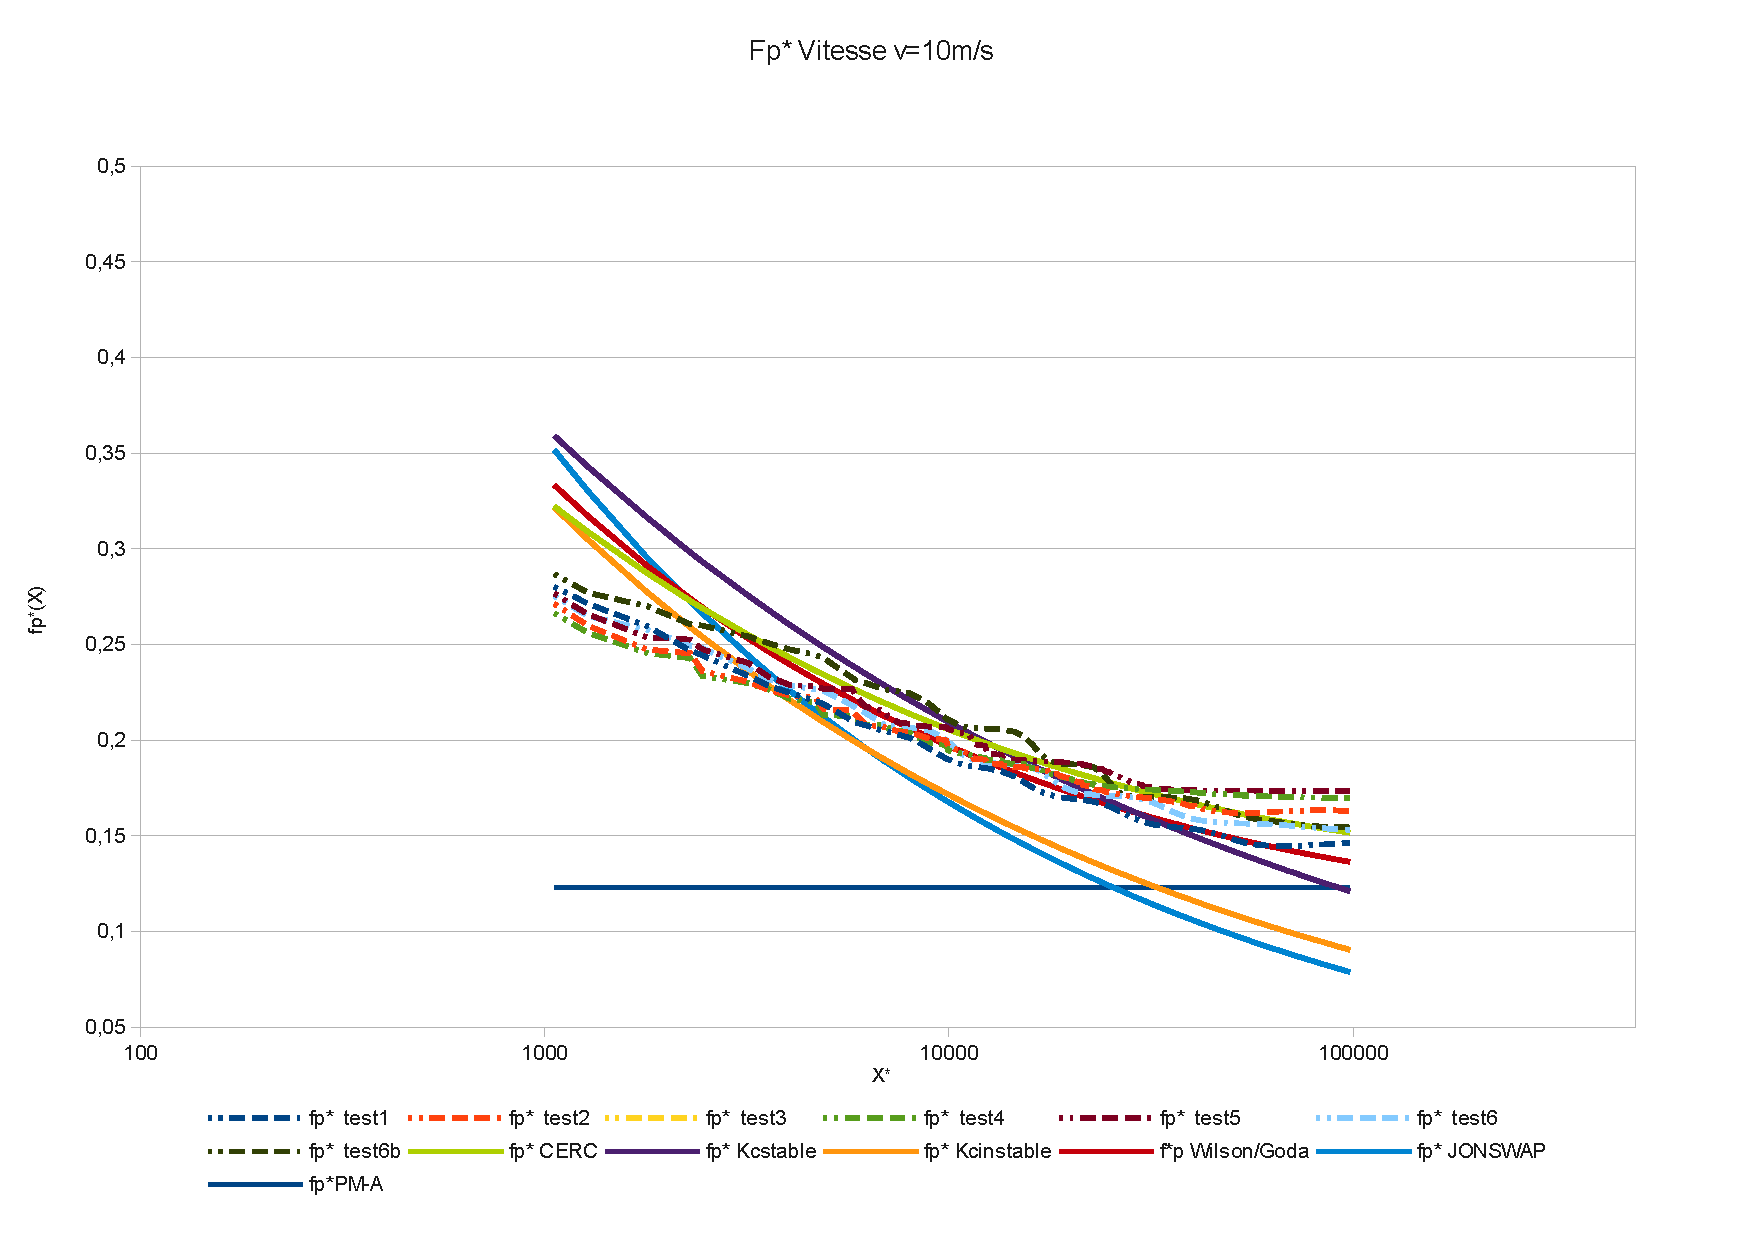
\includegraphics[width=0.5\textwidth]{fpv10id.pdf}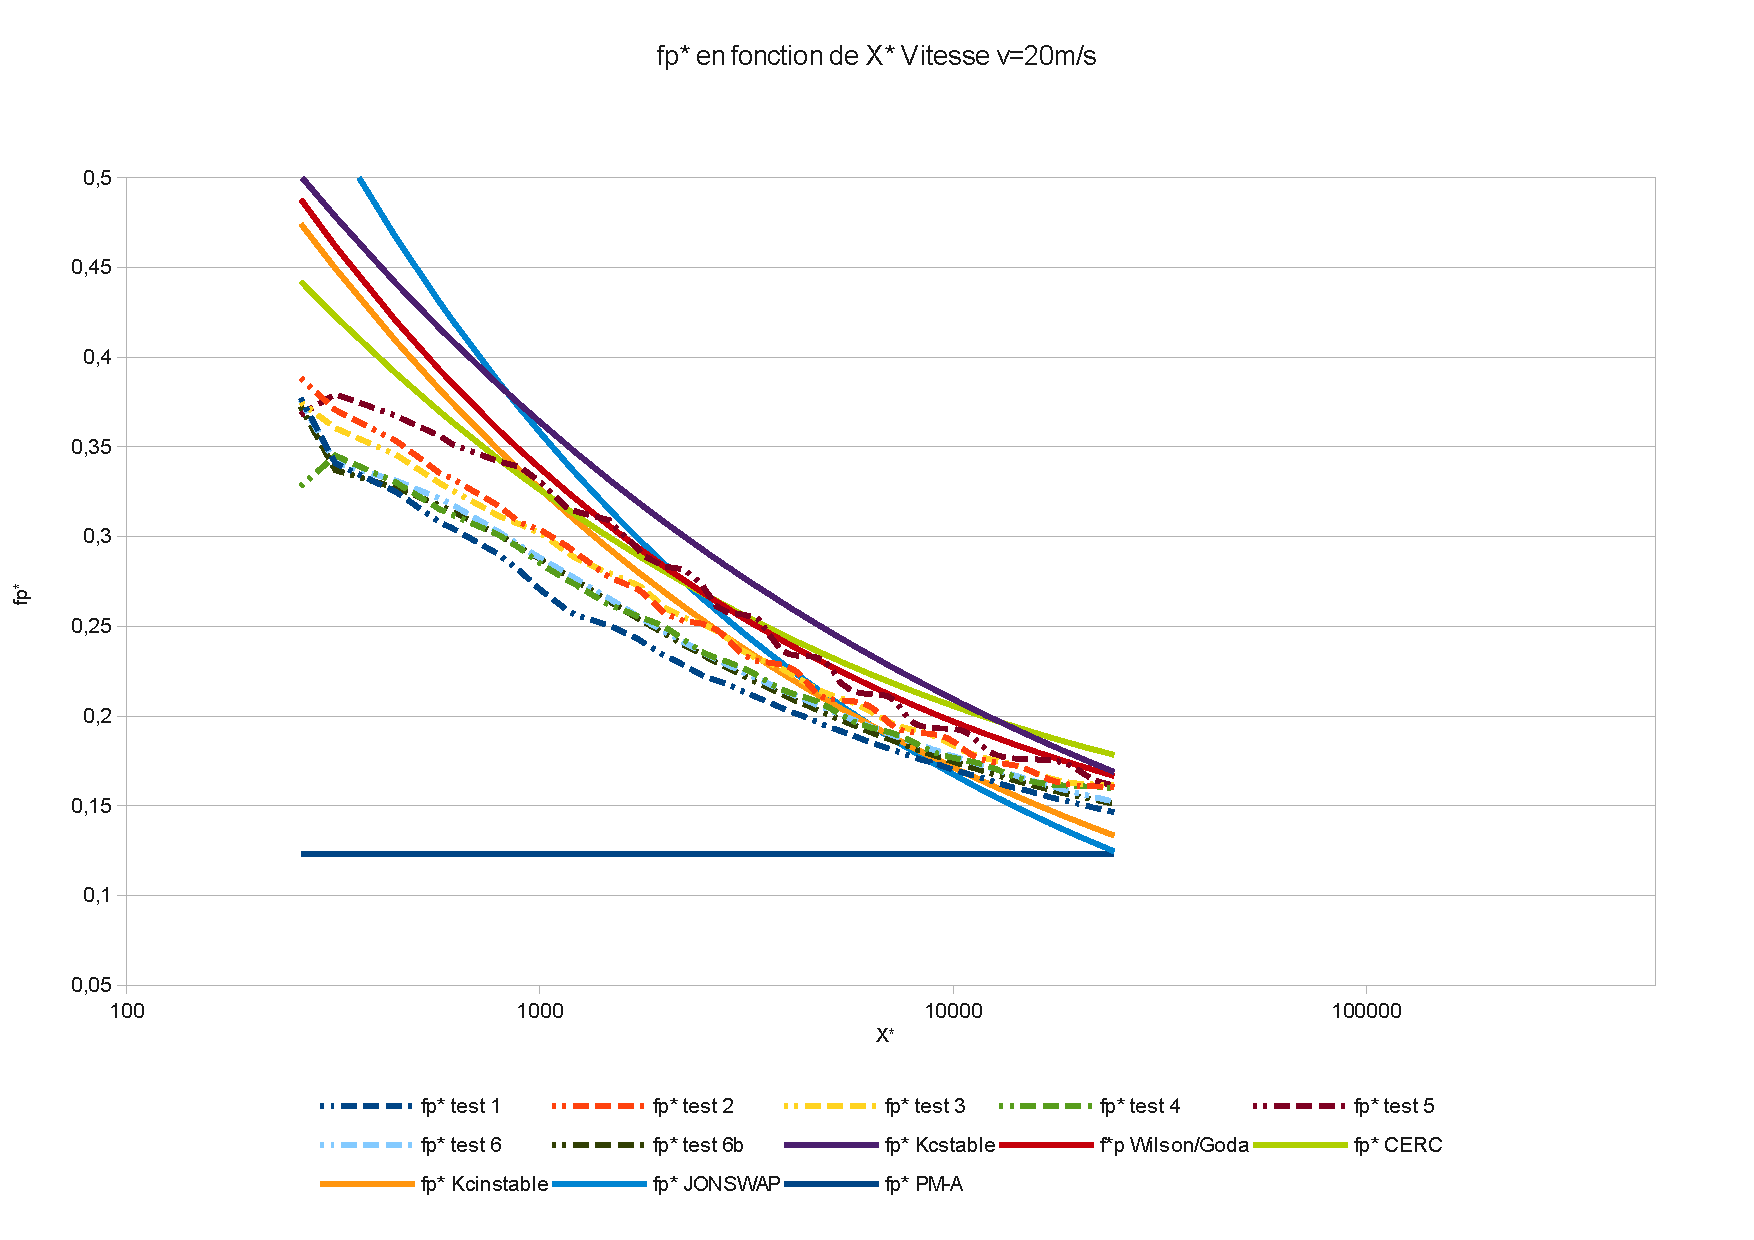
\includegraphics[width=0.5\textwidth]{fpv20id.pdf}\\
      \caption{Comparaison of normalized Variance M0* and normalized peak frequencies fp* for U10 = 10m/s (left) and 20m/s (right), m0* MP-A and fp* PM-A are , respectively, the variance and the peak frequency limits given by the revisited Pierson-Moskowitz formula from Alves (2003)}
\end{figure}
\begin{itemize}
\item Non-dimensionnal Fetch : $x* = \frac{g x}{U_{10}^2}$
\item Non-dimensionnal variance : $m_{0}* = \frac{g^2 m_{0}}{U_{10}^4}$
\item Non-dimensionnal peak frequency : $f_{p}* = \frac{U_{10} f_{p}}{g}$
\end{itemize}
Where $U_{10}$ is the wind velocity at 10 meters from the sea.\\

Figure 4 shows the different results obtained. Generally, all tests give correct results, and stay close to the CERC, Wilson \& Goda and Kahma \& Calkoen curves.\\
The wind impact can be seen by two different behaviours. Indeed, for a 10m/s wind, the results are really close to the empirical formula at small fetches. As the fetch grows, the differences between the models increrase, and the curves began to stray from the empirical formulas. In this case, the models of tests 1, 6 and 6b give the best results. At 20m/s, a different behaviour is noticed : at small fetch the results are quite different from the empirical curves and it is only when the fetch grows that they match well with the empirical formula. In this case it is the model of test 5 which gives the best results. It can be concluded that there is a range where TOMAWAC results are really correct whatever the models used. For strong winds, an exact resolution of the quadruplet transfers, Snyder's wind generation model and Westhuysen white capping model (test 5) give better results at small fetch. \\
Thus, the analysis of Figure 4 shows a good matching between the  TOMAWAC wave simulations and the empirical formulas. A comparison was also done with the revisited Pierson-Moskowitz asymptotic limits from Alves and Banner (2003) for fully developed wind waves, the $U_{10}$-scaled asymptotes is added on Figure 4.The formula gives : 
\[\epsilon = (4.02 \pm 0.62)*10^{-3}\]
\[\nu = (1.23 \pm 0.08)* 10^{-1}\]
 It seems that the non-dimensional peak frequency $f_p*$ is a little bit over-estimated and the non-dimensional variance is a bit underestimated. Indeed, the empirical formula given by CERC (1984), which is used as a criterion for fully developed seas, to calculate the minimum fetch during the minimum duration (48h), is : $\frac{t_{min} g}{U_{10}} = 68.8 (\frac{X_{min} g}{U_{10}^2})^{0.67}$. Applying this formula we found that the fully developed seas is reached around $1 117 km$ for a 10 m/s wind and around $1 672 km$ for a 20 m/s wind. Thus, the fully developed sea may not be entirely reached at our last point ($X_{10} = 1000km$) and which may explain the growth of the variance spectrum for some of the tests (see next section). 

\subsection{Variance spectrum for a constant wind}
In this section, we look at the development of the variance spectrum $E(f)$ along the fetch.
\[ E(f) = \int_{0}^{2\pi} F(f,\theta )d\theta
\]
The spectra are worked out for different points of fetch and for two wind speeds (10m/s and 20m/s):\\
\begin{center}
\begin{tabular}{c|c}
Points & fetch\\
\hline
Point 1 & 25 km \\
Point 2 & 50 km \\
Point 3 & 100 km \\
Point 4 & 150 km \\
Point 5 & 200 km\\
Point 6 & 300 km \\
Point 7 & 400 km \\
Point 8 & 800 km\\
Point 9 & 750 km\\
Point 10 & 1000 km\\
\end{tabular}\\
\end{center}
Dimensional variance spectrum (not shown here) gives correct results with a big growth of the peak value with the wind.\\
The non-dimensionnal frequency is defined by : $f* = \frac{U_{10}*f}{g}$.\\
and the variance spectra are normalised by the peak value of the Pierson-Moskowitz spectrum, which corresponds to the steady state :\\
$E_{PM}(f_{PM}) = \frac{\alpha g^2}{(2\pi)^4 f_{PM}^5} exp(-5/4)$ with $f_{PM}=\frac{0.13 g}{U_{10}}$ and the Philipp's constant $\alpha = 0.0081$\\
\begin{figure}[h!]
  \begin{tabular}{cc}
  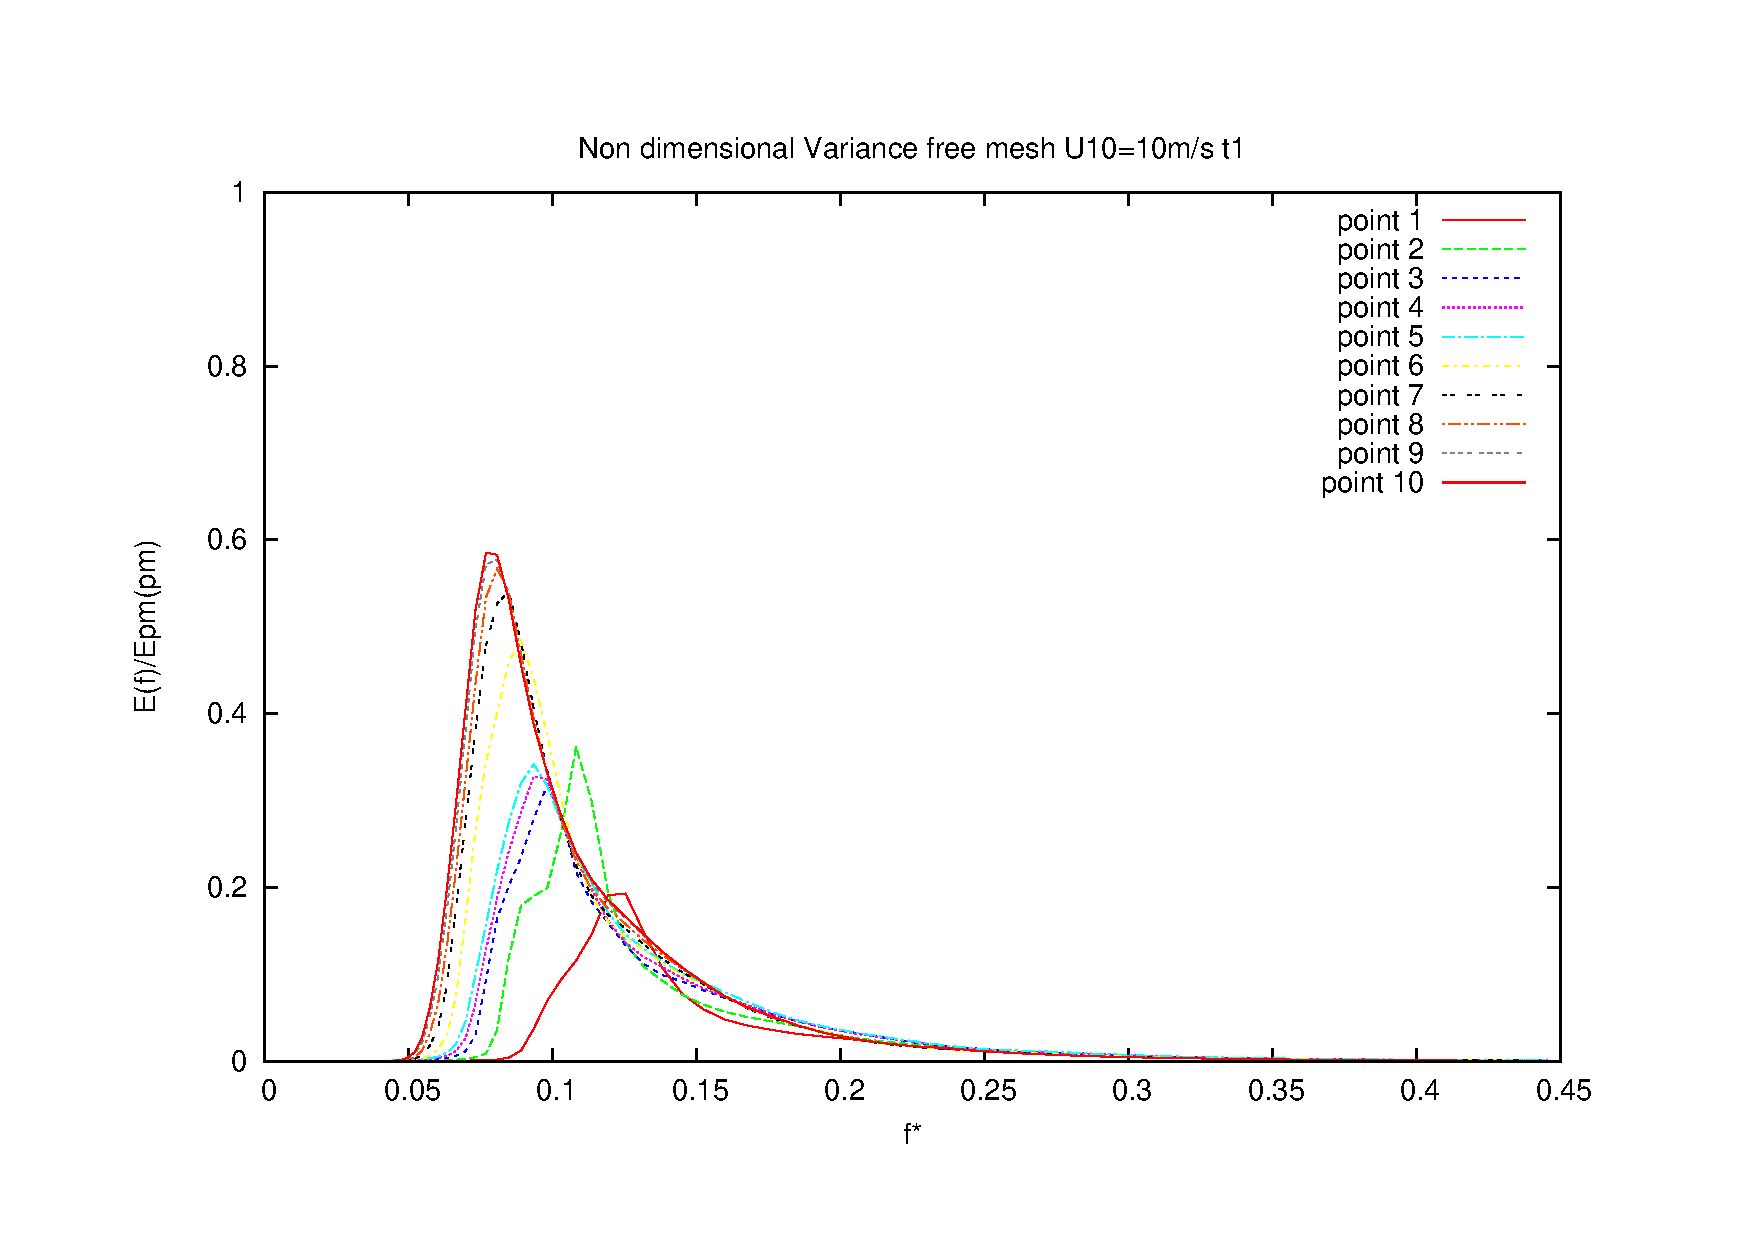
\includegraphics[width=0.5\textwidth]{variance_ad_free_mesh_t1_v10.pdf} & 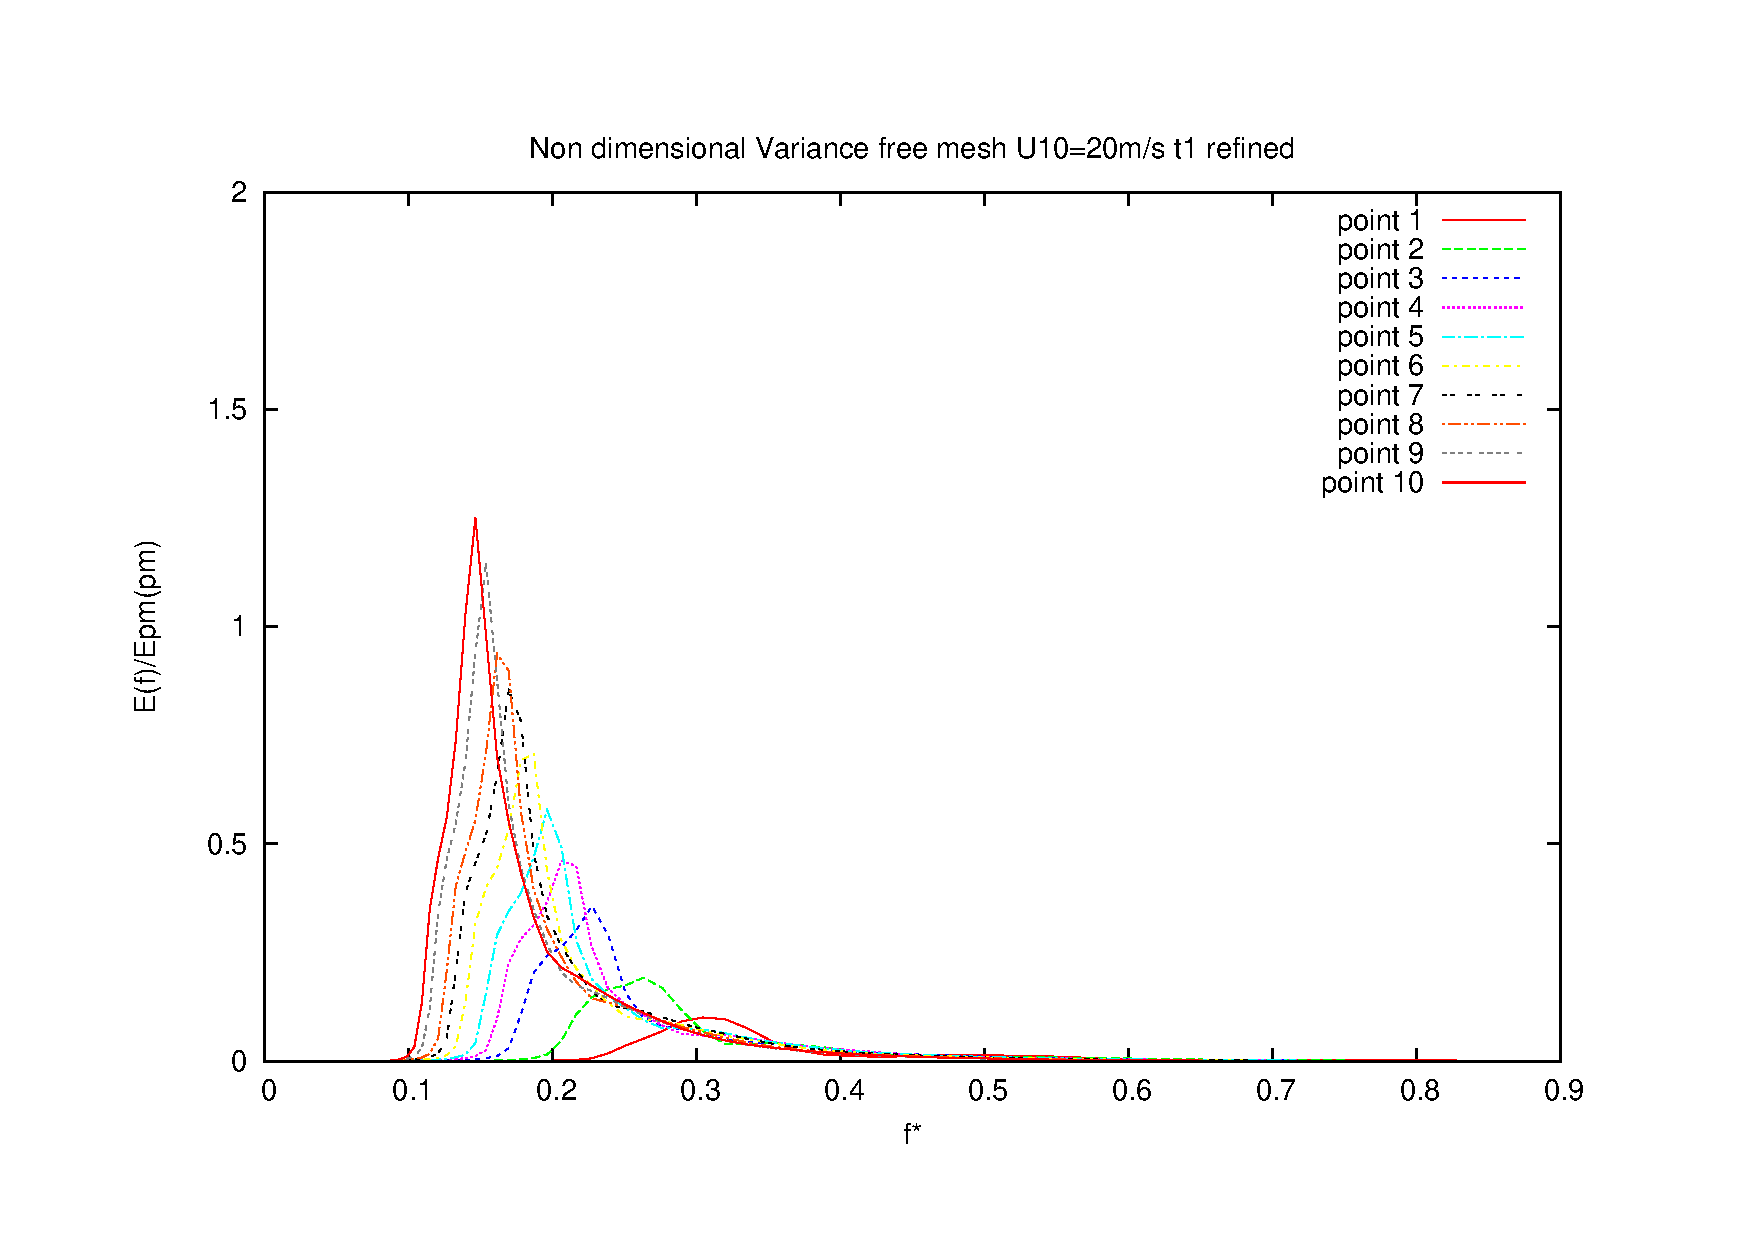
\includegraphics[width=0.5\textwidth]{freemesh/Profondeurinfinie/test1/variance_ad_free_mesh_t1_fine_v20.pdf}\\
    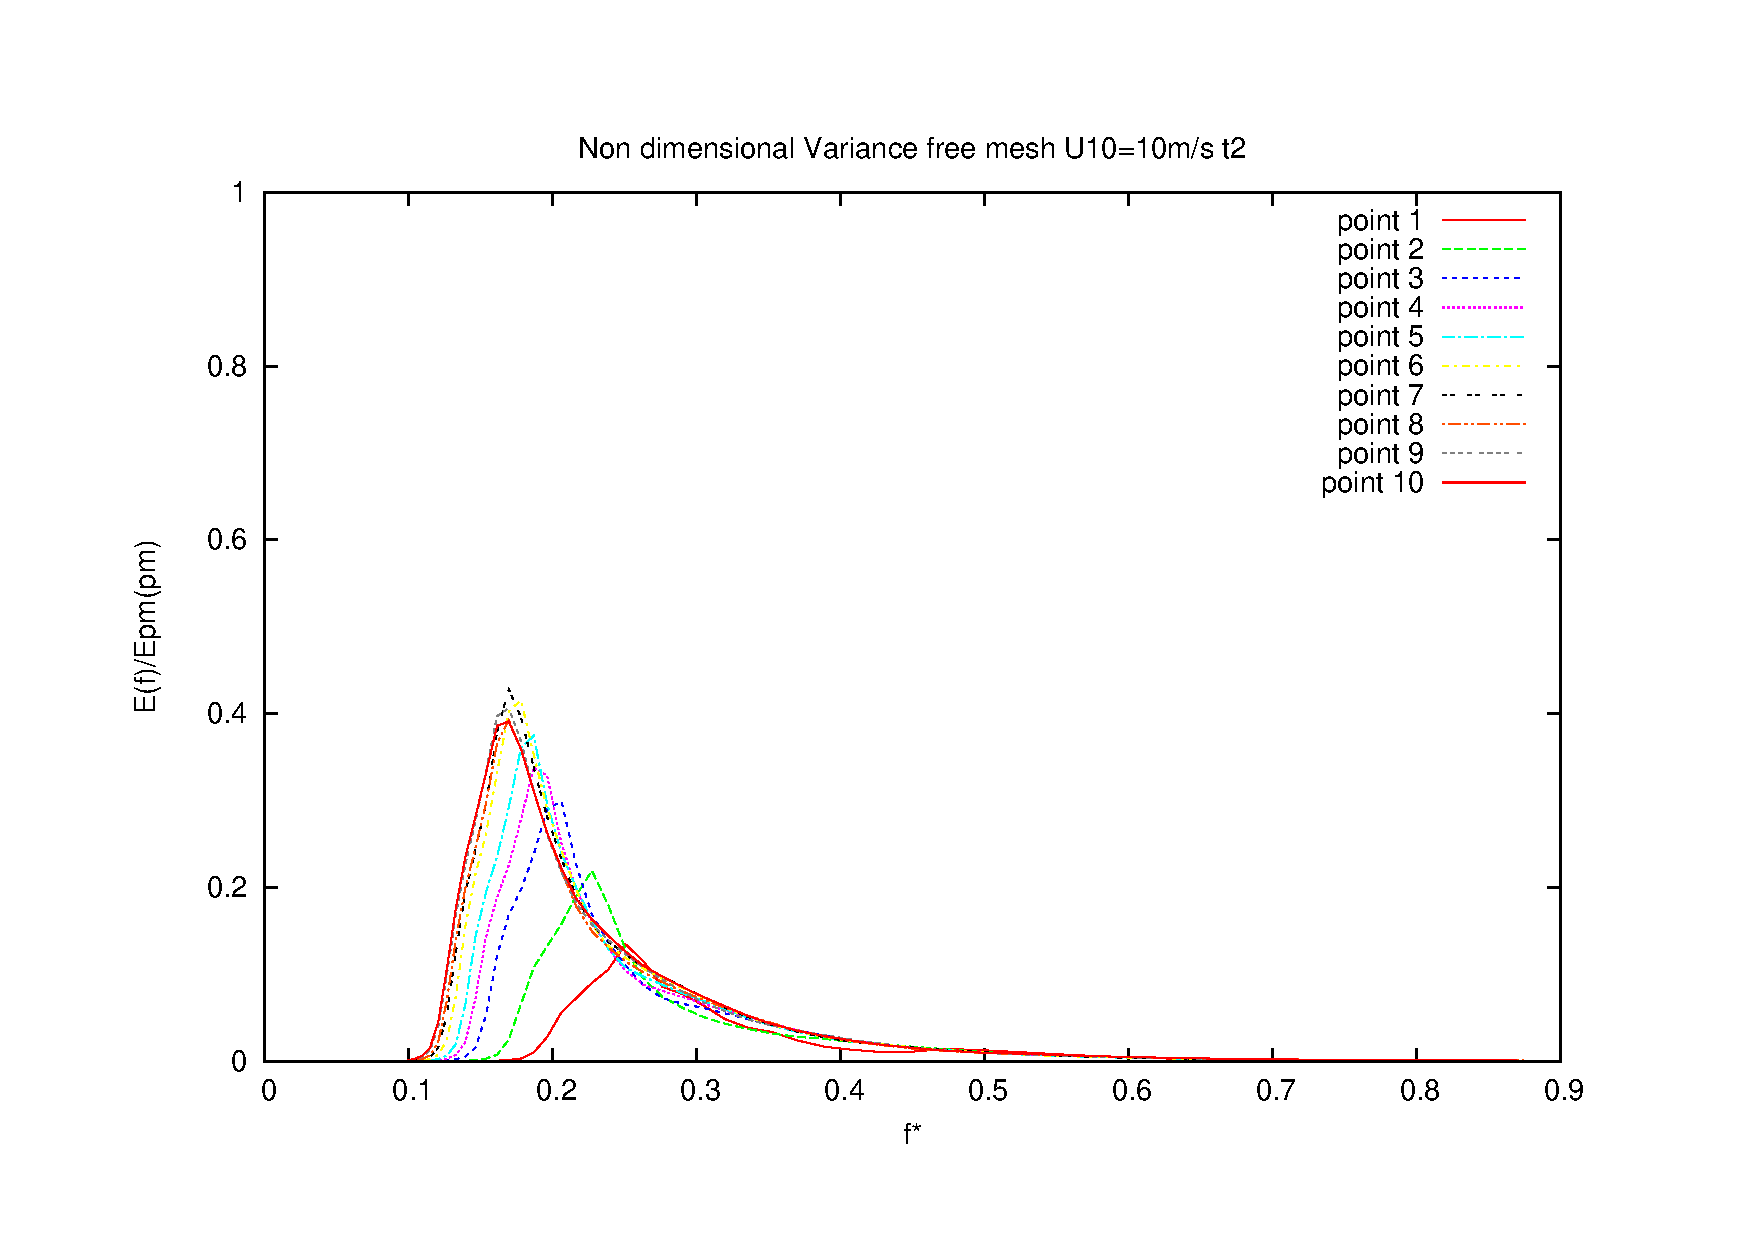
\includegraphics[width=0.5\textwidth]{variance_ad_free_mesh_t2_v10.pdf} & 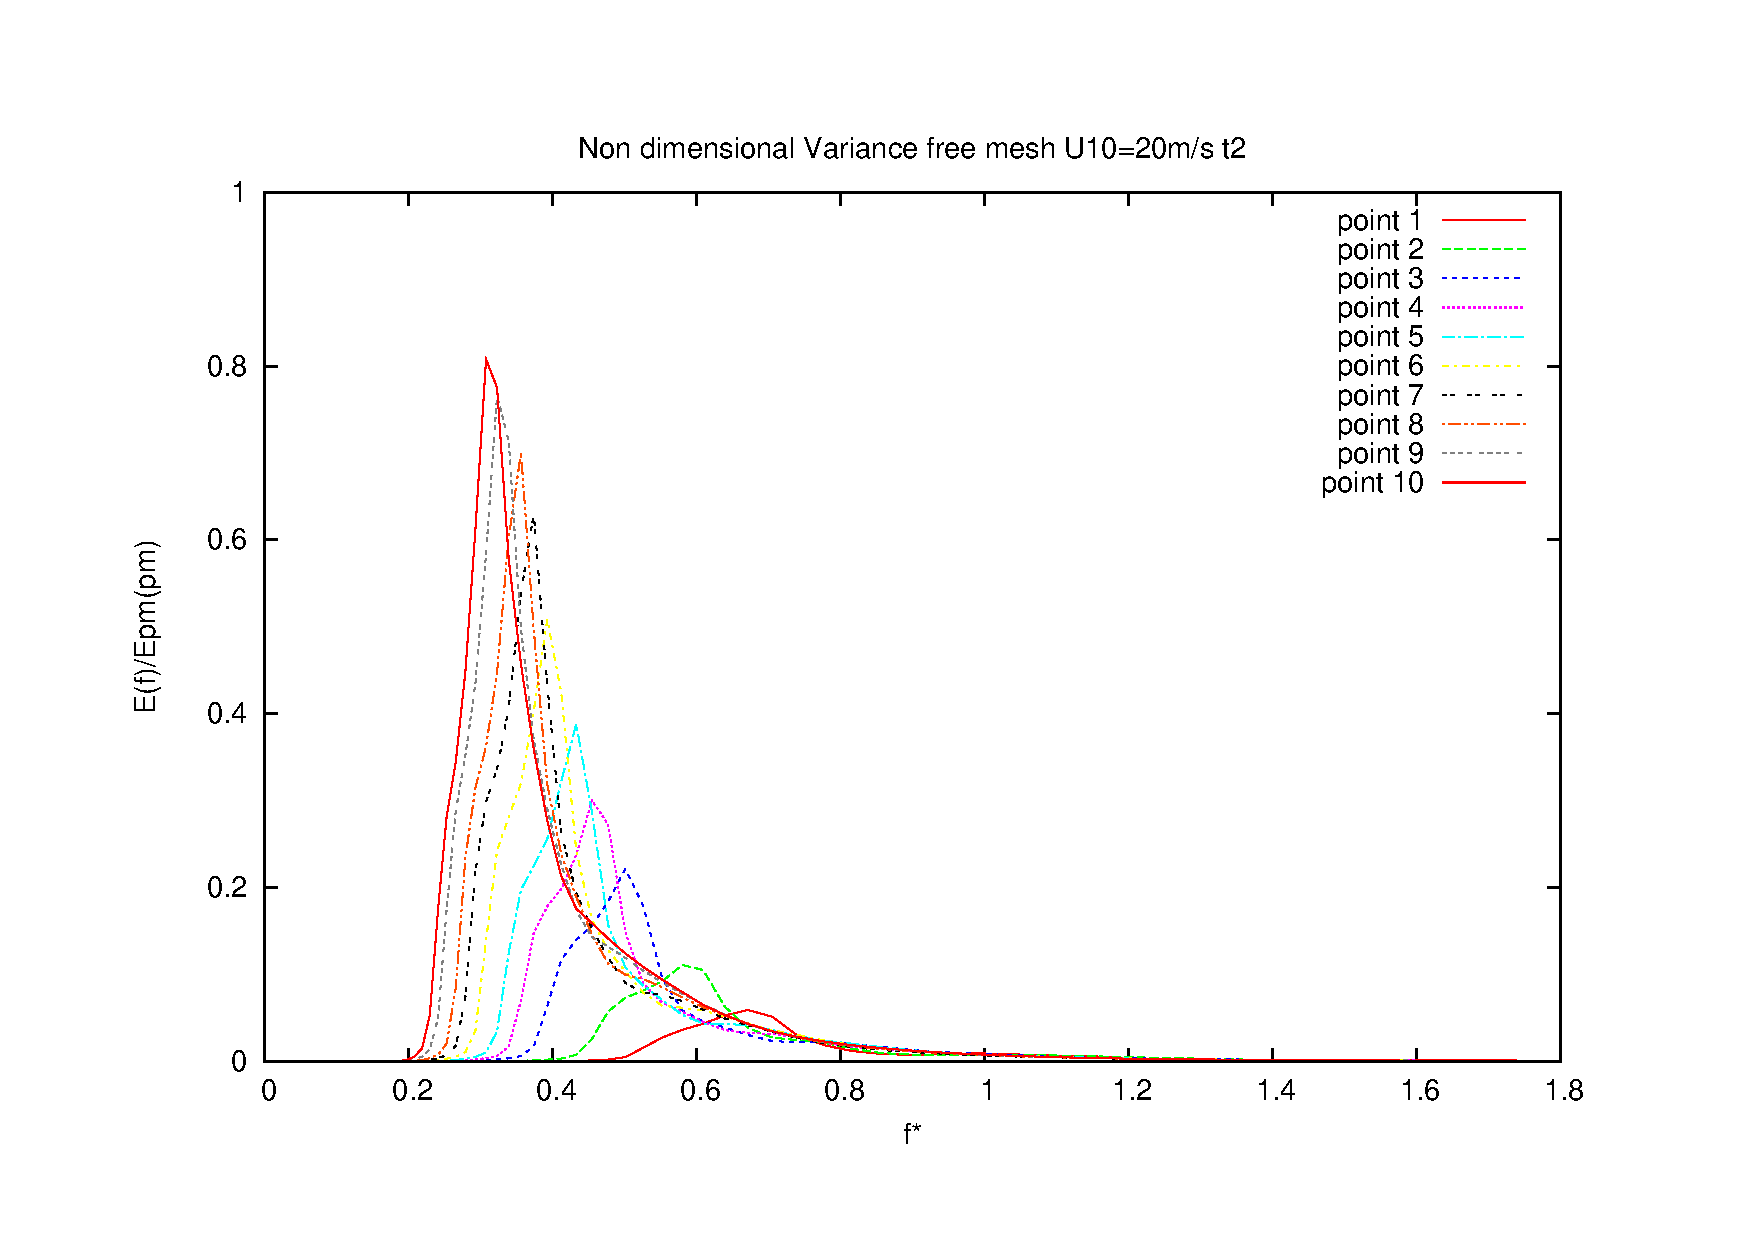
\includegraphics[width=0.5\textwidth]{freemesh/Profondeurinfinie/test2/variance_ad_free_mesh_t2_v20.pdf}\\
      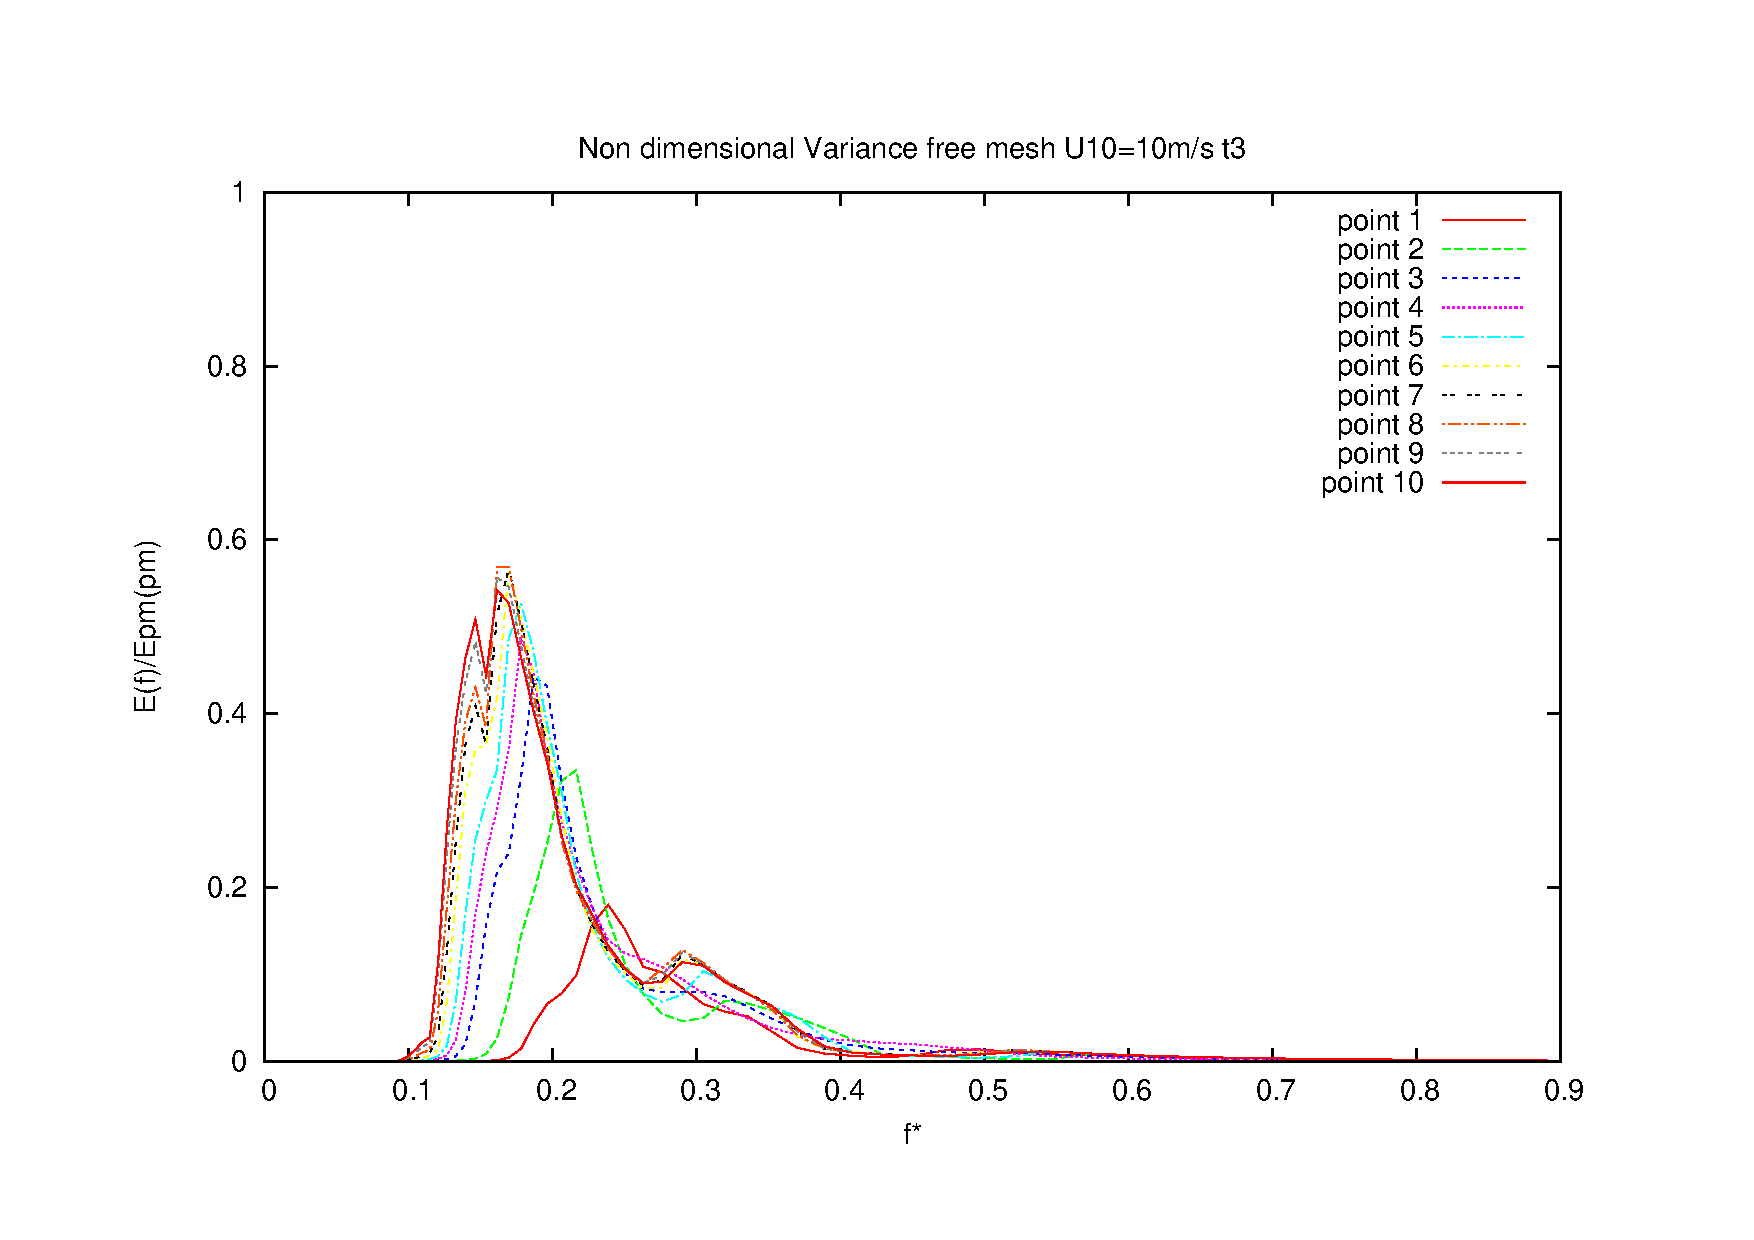
\includegraphics[width=0.5\textwidth]{variance_ad_free_mesh_t3_v10.pdf} & 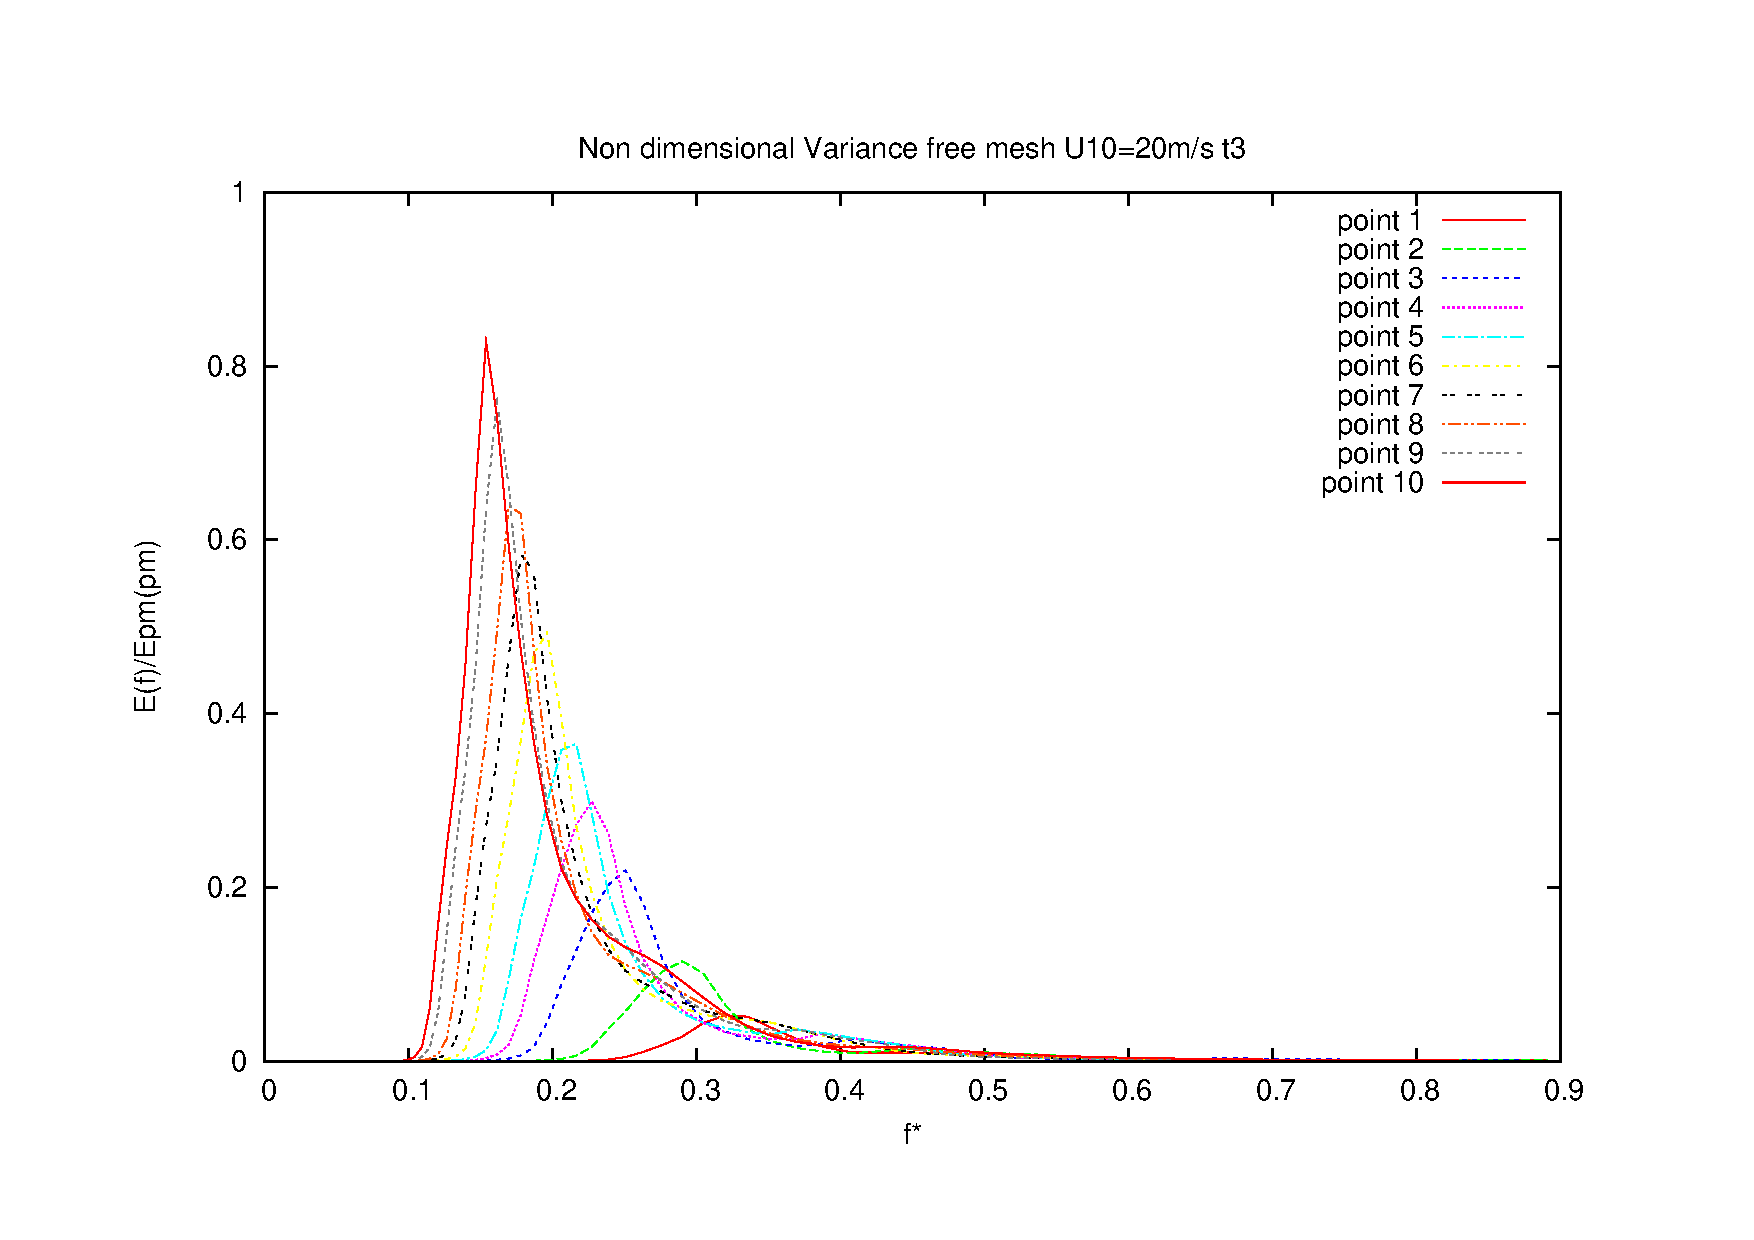
\includegraphics[width=0.5\textwidth]{freemesh/Profondeurinfinie/test3/variance_ad_free_mesh_t3_v20.pdf}\\
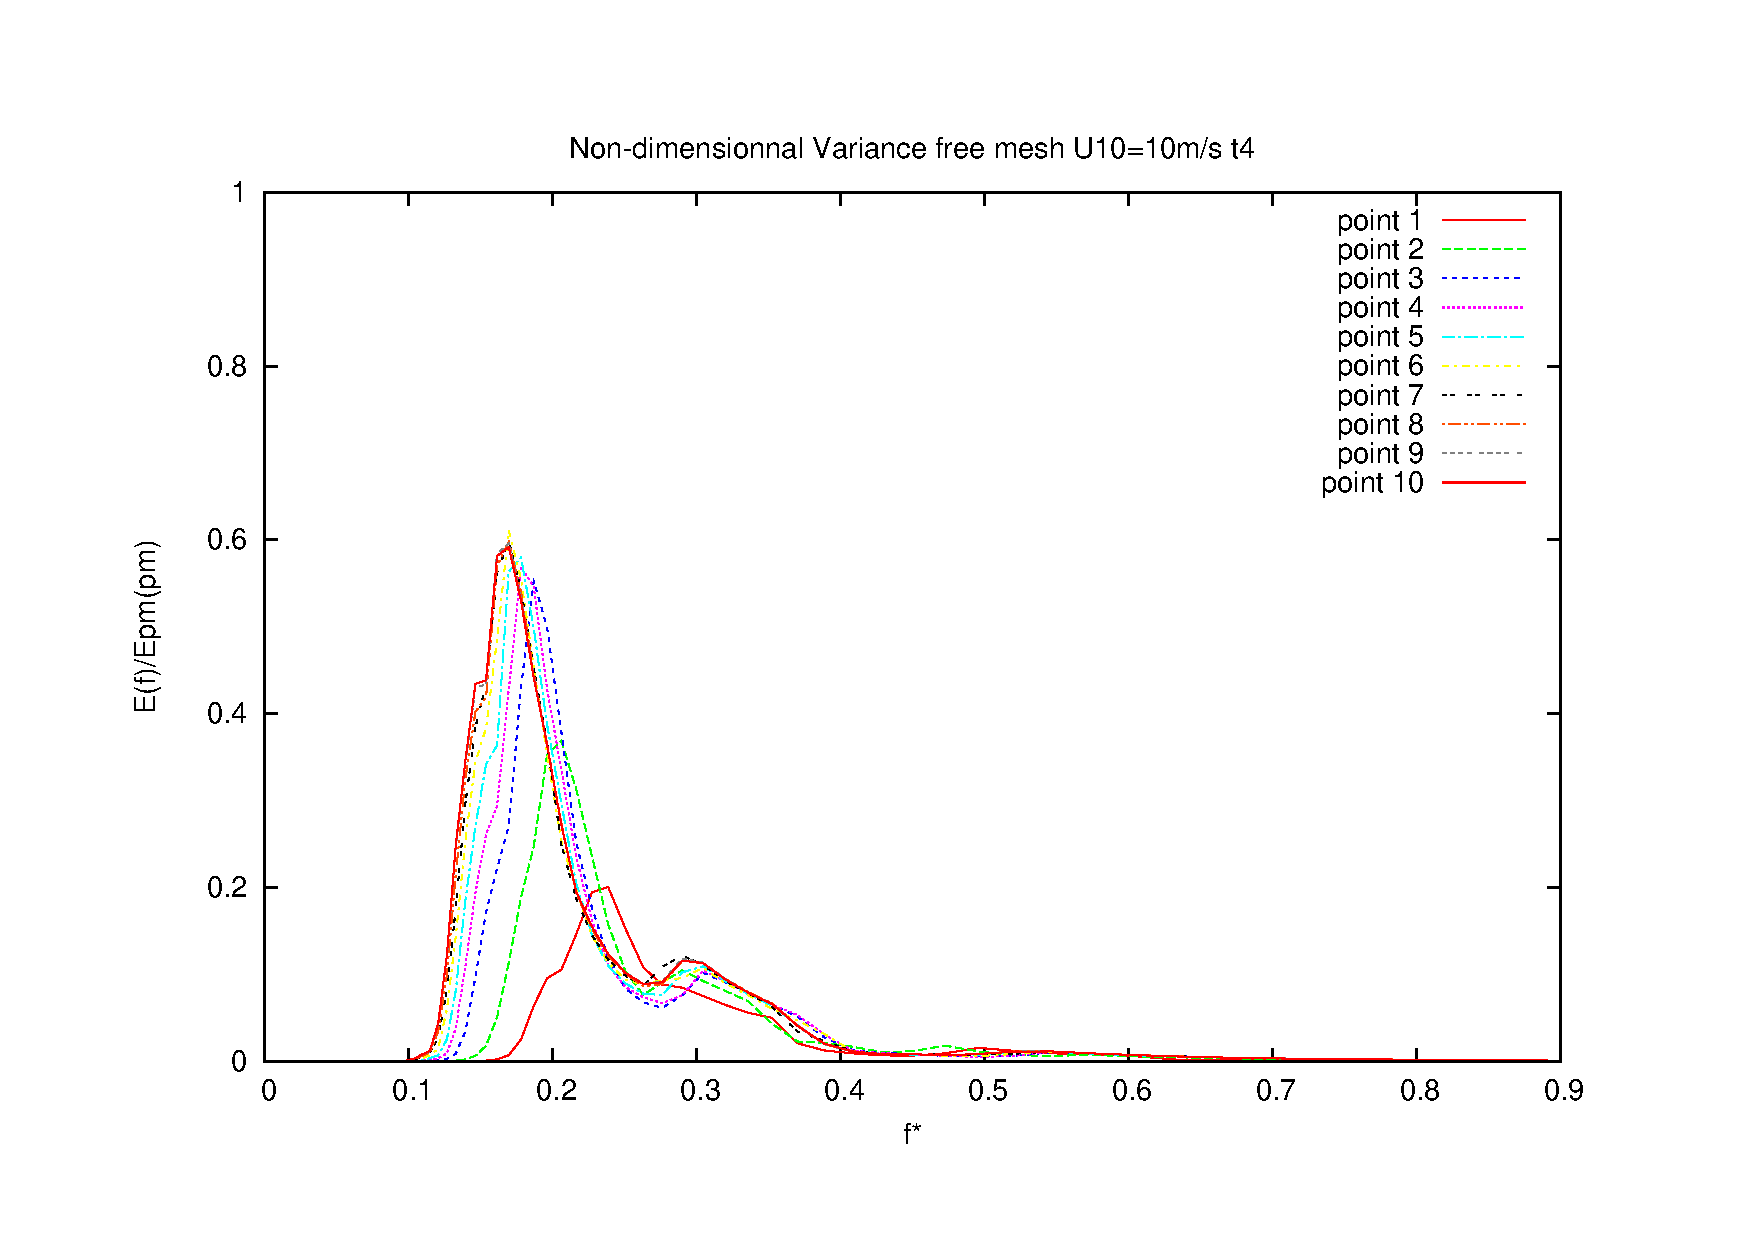
\includegraphics[width=0.5\textwidth]{variance_ad_free_mesh_t4_v10.pdf} & 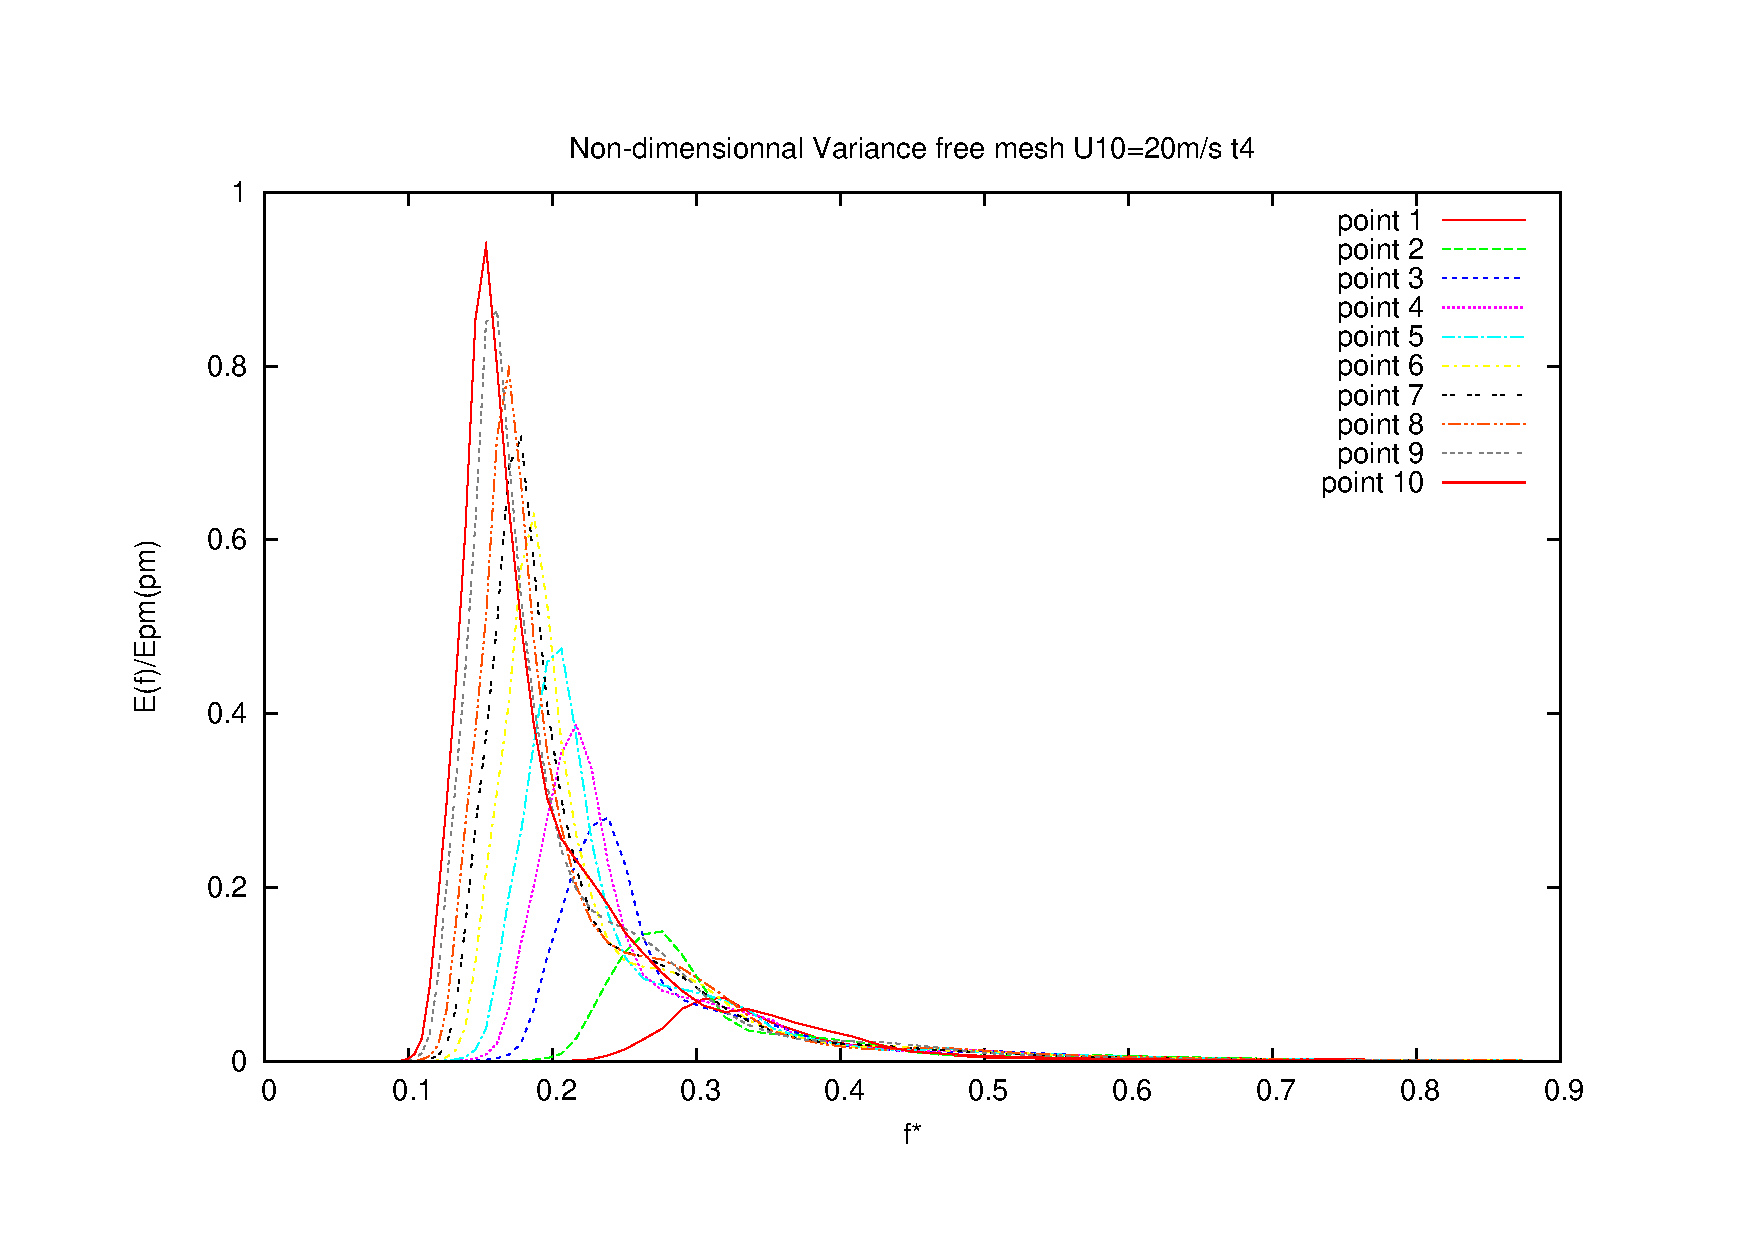
\includegraphics[width=0.5\textwidth]{freemesh/Profondeurinfinie/test4/variance_ad_free_mesh_t4_v20.pdf}\\
        \end{tabular}\end{figure}\begin{figure}[h!]
          \begin{tabular}{cc}
          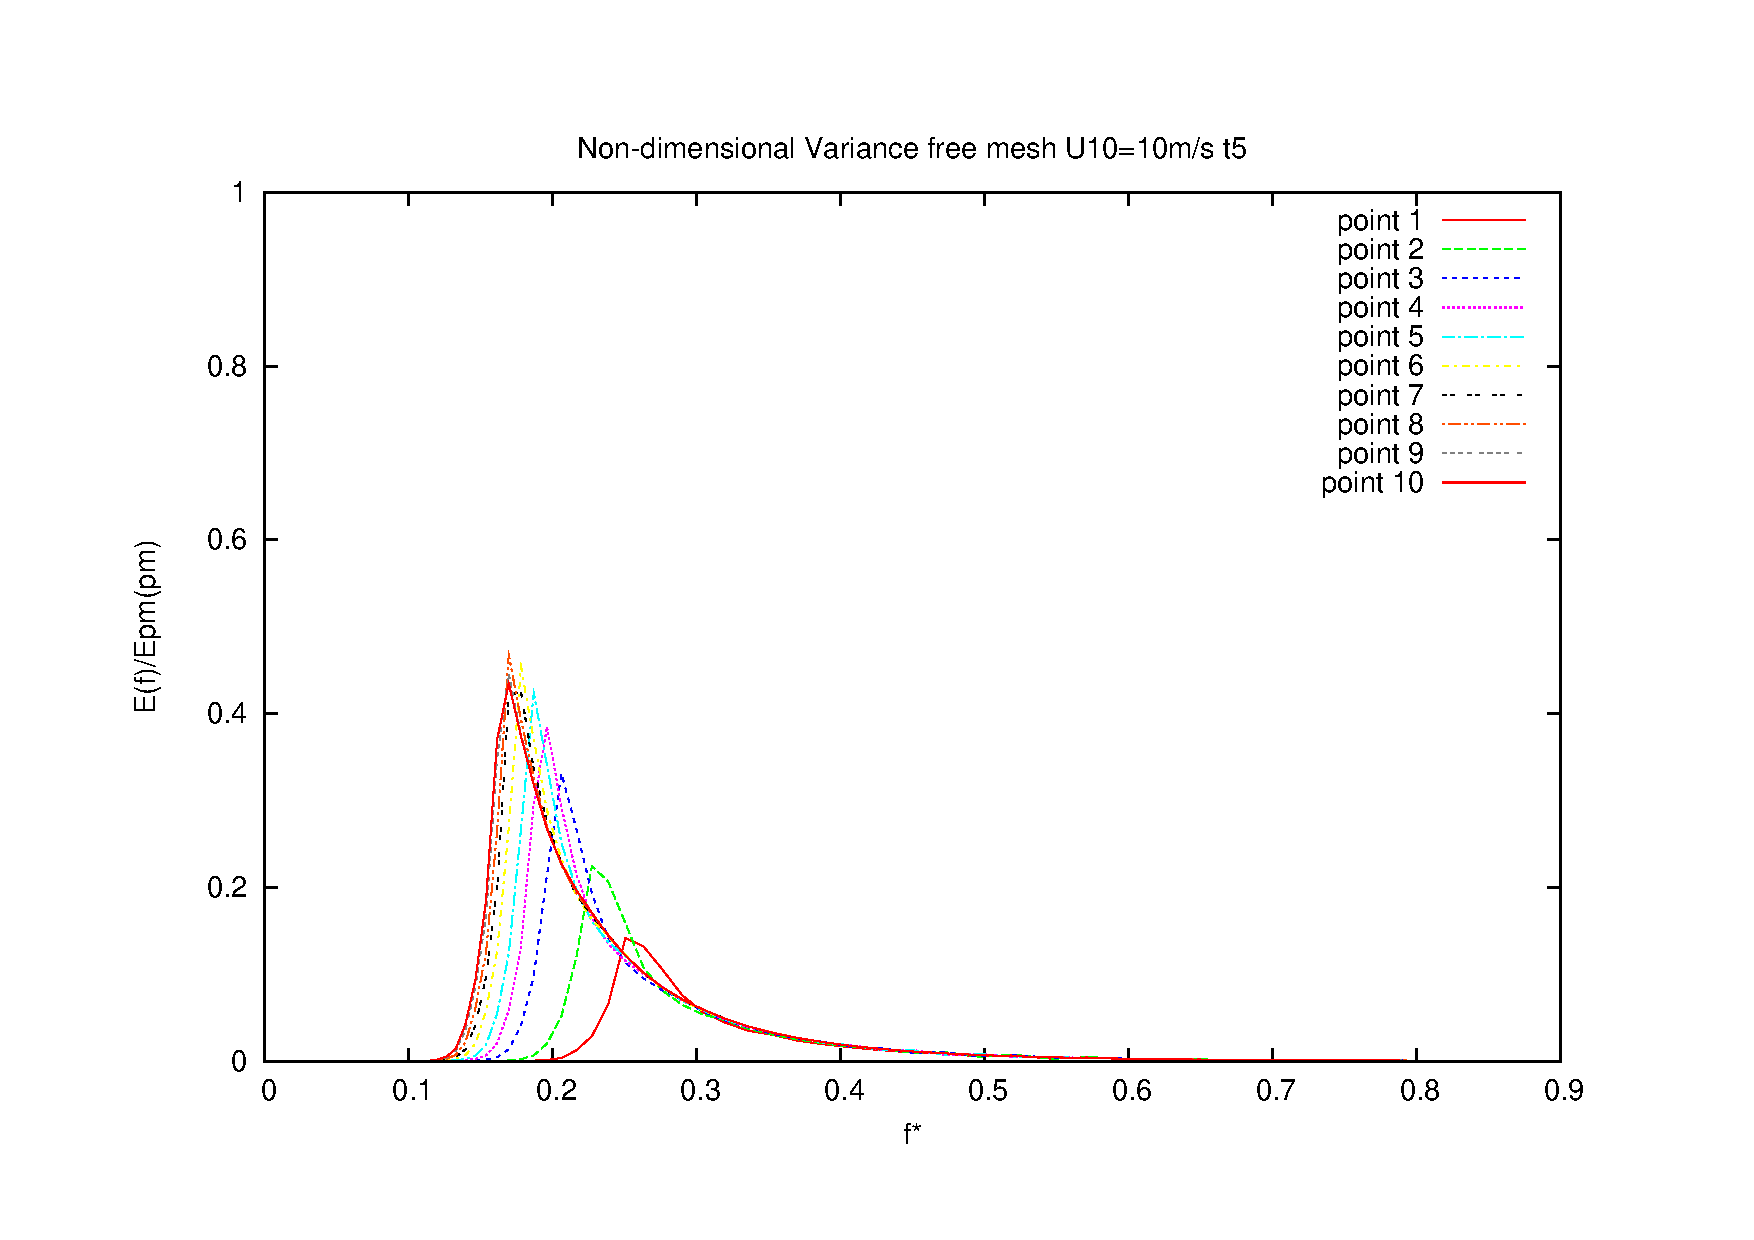
\includegraphics[width=0.5\textwidth]{variance_ad_free_mesh_t5_v10.pdf} & 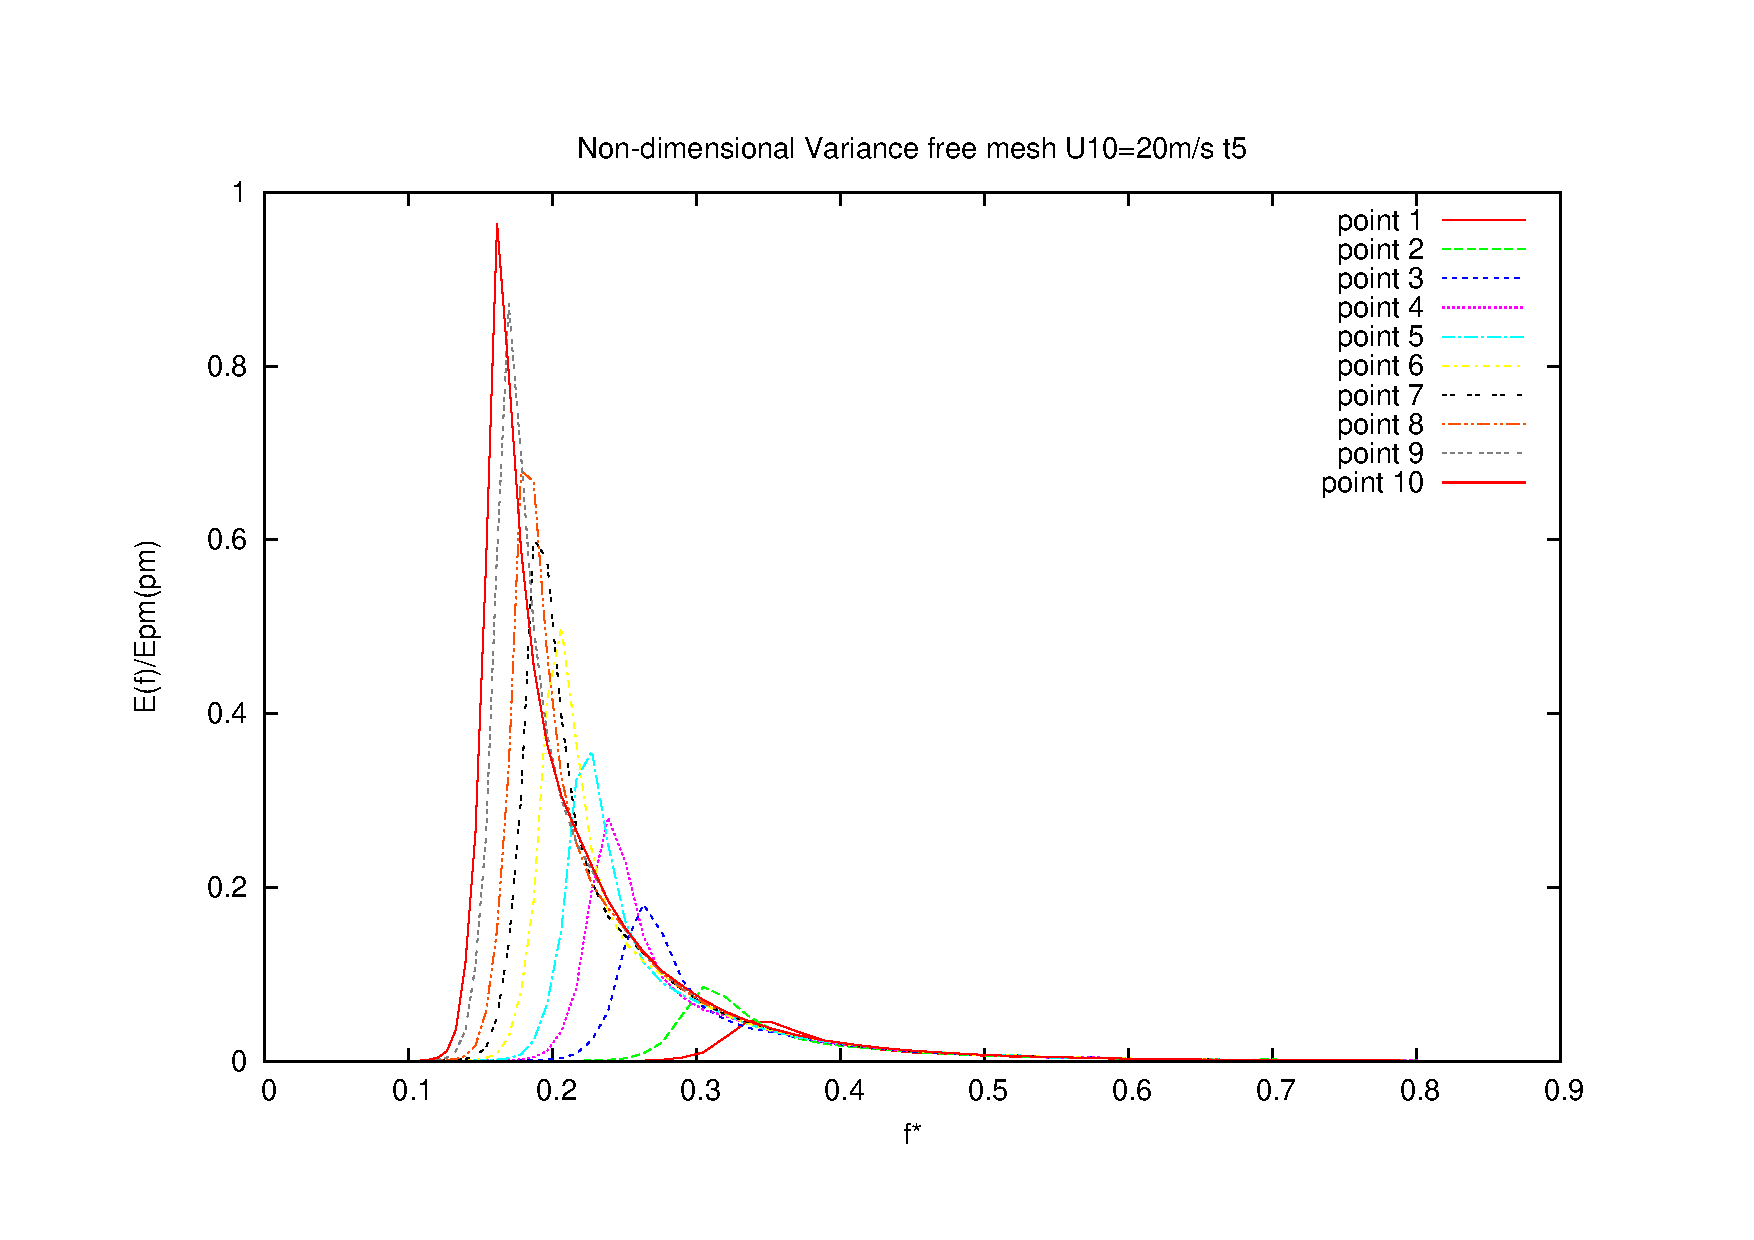
\includegraphics[width=0.5\textwidth]{freemesh/Profondeurinfinie/test5/variance_ad_free_mesh_t5_v20.pdf}\\\\
  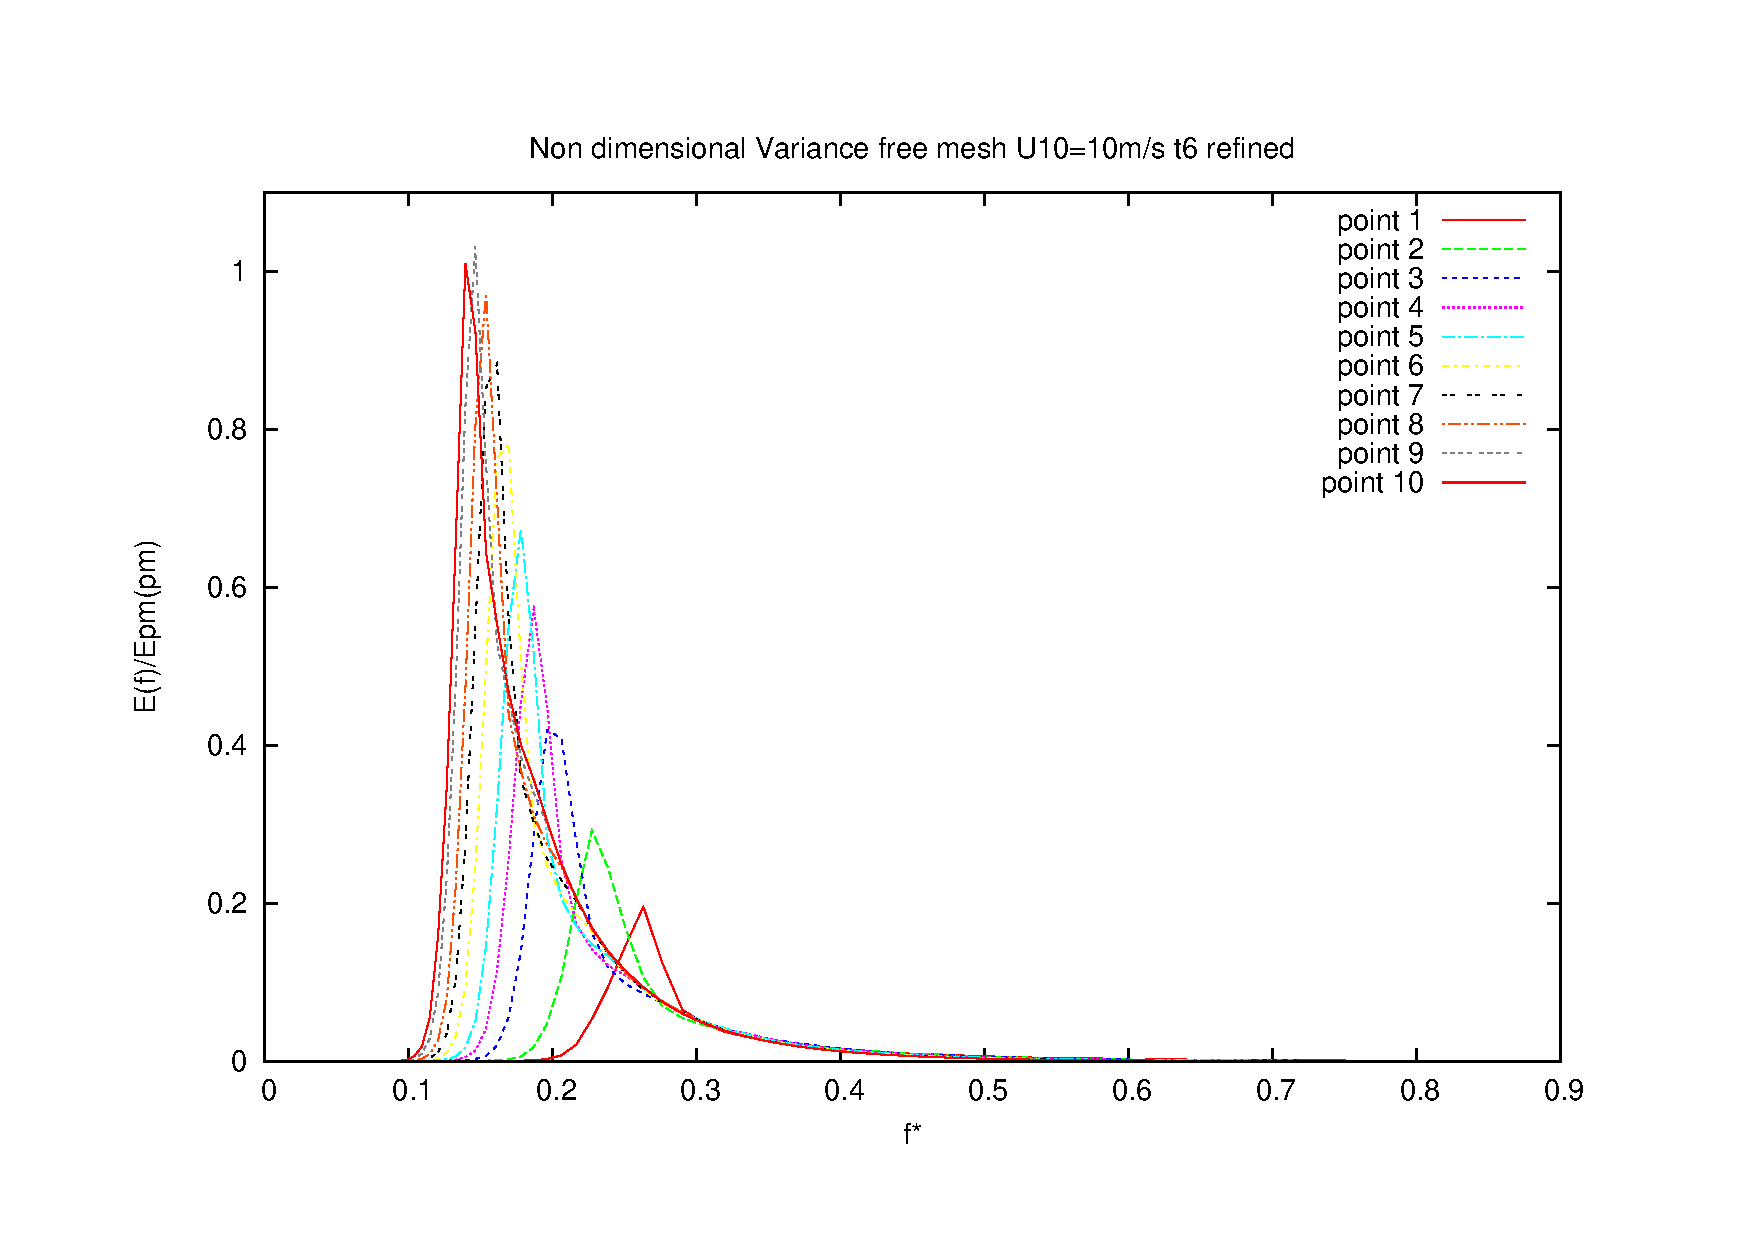
\includegraphics[width=0.5\textwidth]{variance_ad_free_mesh_t6_v10.pdf} & 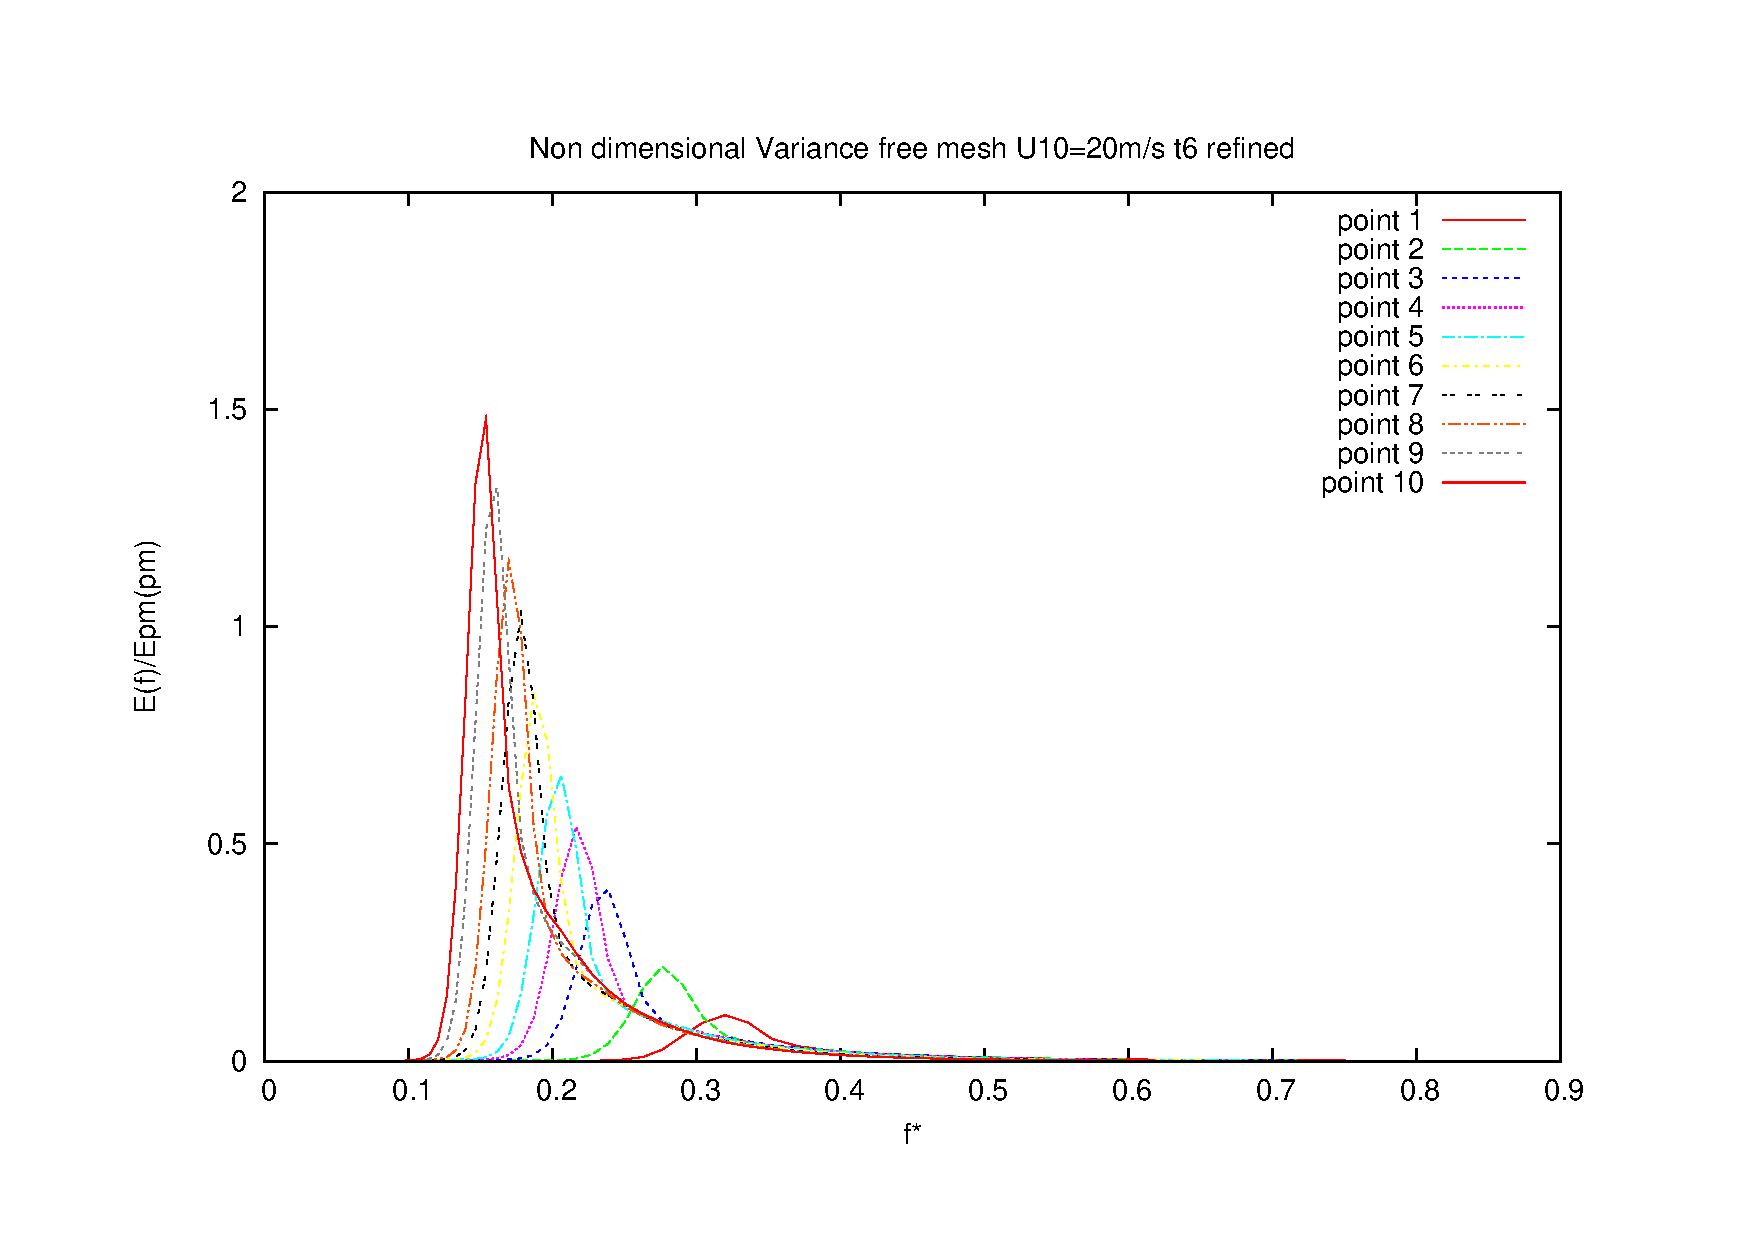
\includegraphics[width=0.5\textwidth]{freemesh/Profondeurinfinie/test6/variance_ad_free_mesh_t6_fine_v20.pdf}\\
    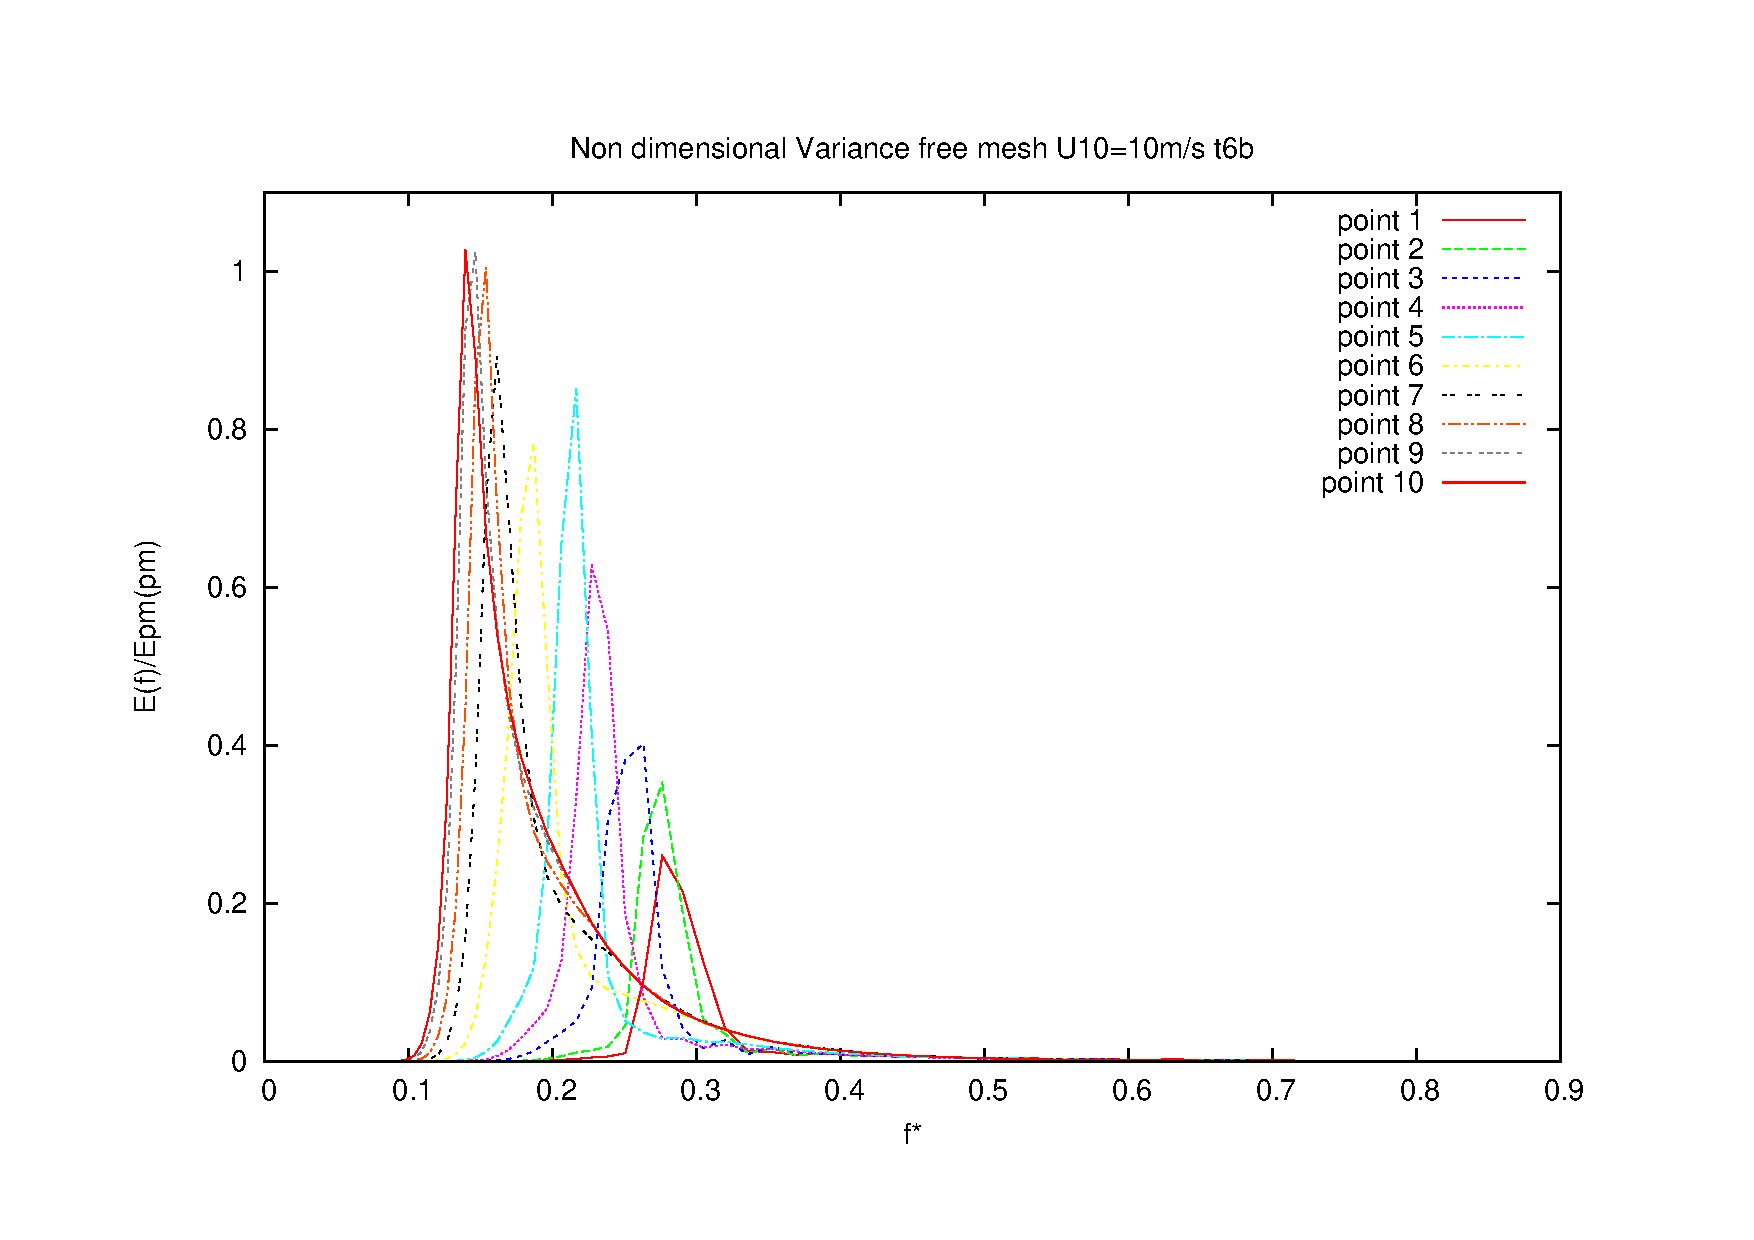
\includegraphics[width=0.5\textwidth]{variance_ad_free_mesh_t6b_v10.pdf} & 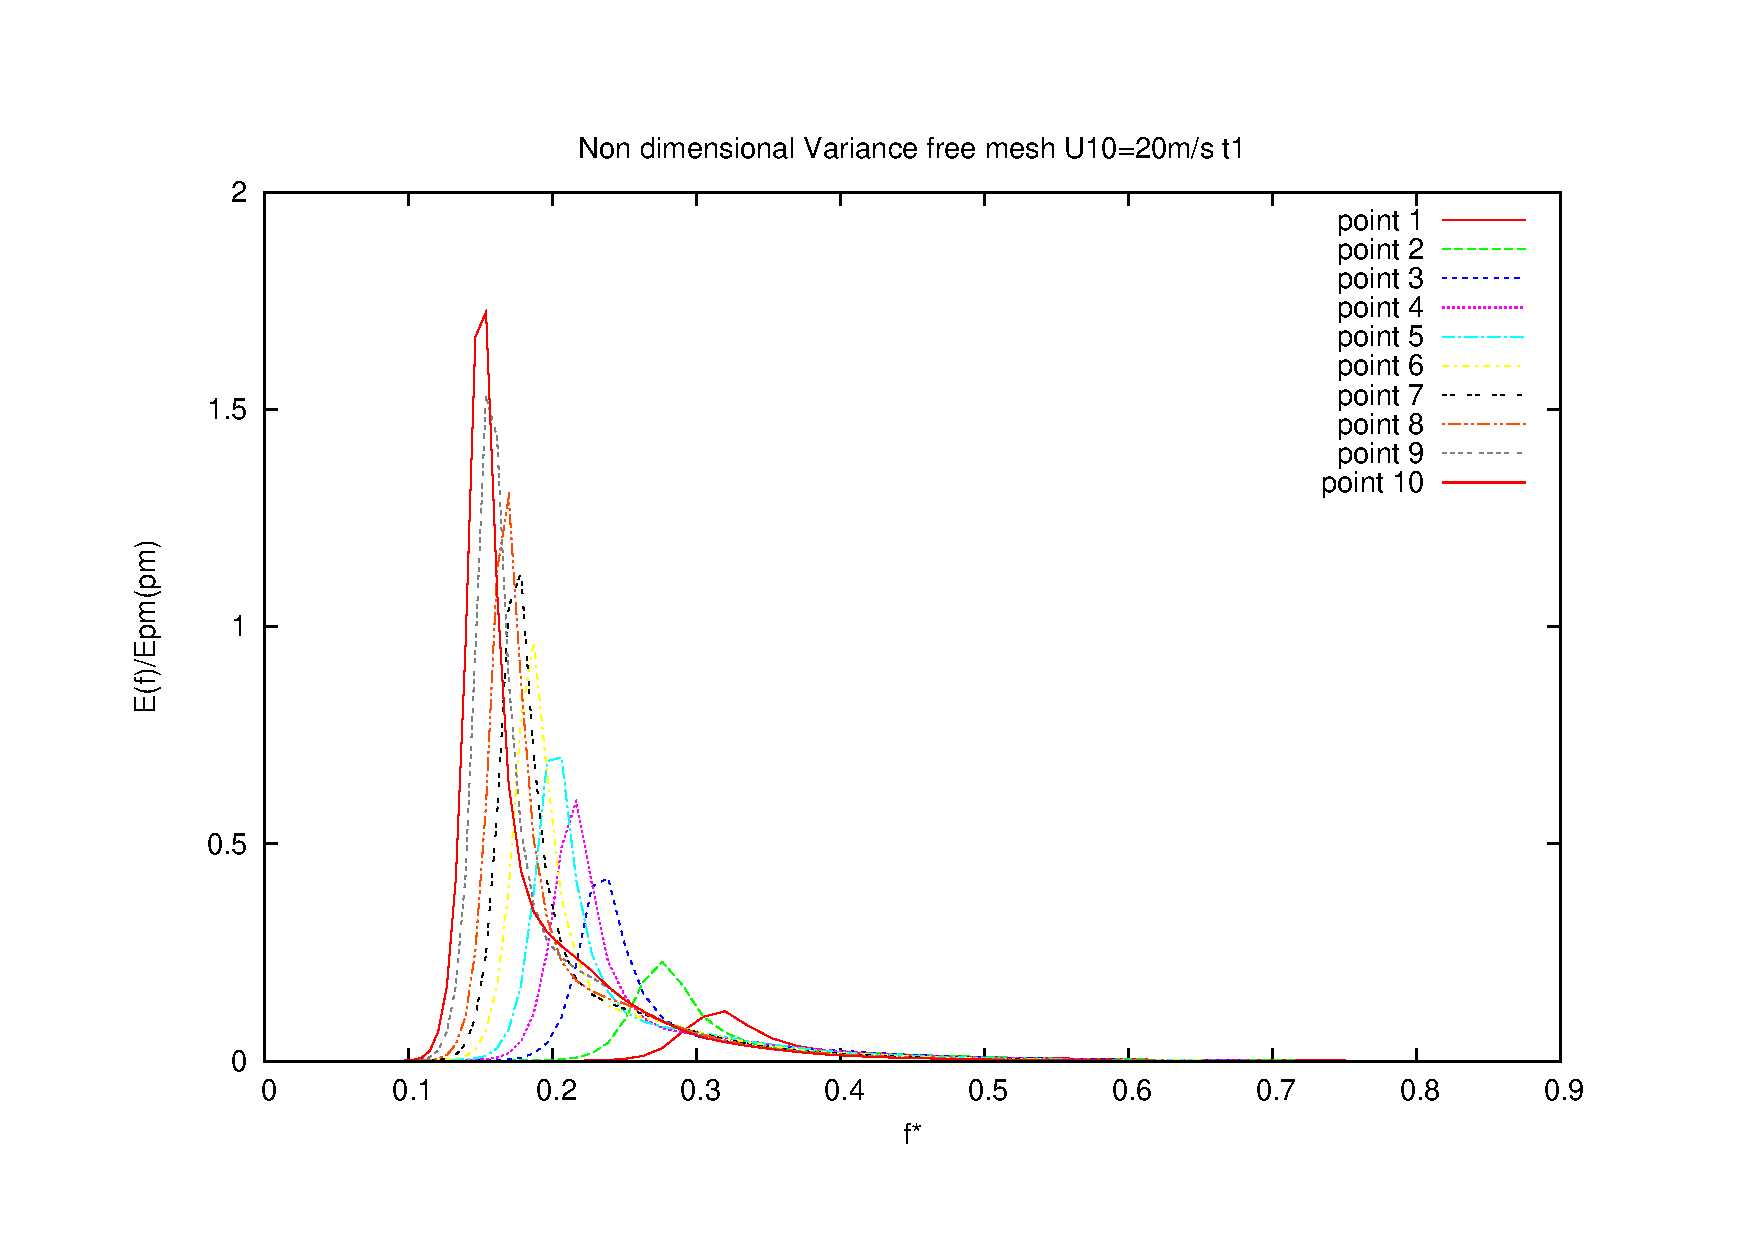
\includegraphics[width=0.5\textwidth]{freemesh/Profondeurinfinie/test6b/variance_ad_free_mesh_t6b_v20.pdf}\\
  \end{tabular}
      \caption{Comparaison of normalized spectrum variance for the different tests and U10 = 10m/s (left) and 20m/s (right).}
\end{figure}
On Figure 5, non-dimensionnal variance spectra can be observed. We can notice that as the fetch grows, the variance spectrum amplitude grows and the peak frequency declines. Moreover, the variance spectrum tends to the Pierson-Moskowitz spectrum for some cases. The exact quadruplet transfers calculation impact can be seen on the test 5, 6 and 6b, the shape of the curve changes, the spectrum is more peaked and the maximum value is higher, and it allows to observe a spectrum peak overstepping the state value predicted by Pierson-Moskowitz formula, it is an overshoot (test 6 for $U10 = 20m/s$ and test 6b).\\
For $U10 = 10m/s$, the last fetch points (points 7, 8, 9 and 10) get really close spectra. We can conclude that from a certain fetch, the fully developed sea state is reached. Althought, for the case $U10 = 20m/s$, the spectrum continues to grow and the overshoot's presence shows that this balance state is not yet reached. Thus, TOMAWAC gives good results which can be improved with the exact GQM quadruplet transfers model.

\subsection{Finite depth TOMAWAC results}
In this section, finite depths are considered : 180m, 60m, 30m, 15m and 5m. In regards of Miche's criterion (1994), excepted for a 5 meters depth and $V = 20m/s$, there is no bathymetric breaking dissipation. All the tests are done for the same generation (Snyder), white capping (Westhuysen) and quadruplet transfer (DIA) models. Figure 6 shows the evolution of the non-dimensional variance along the fetch for the different tests. In order to compare with the CERC (1984) parametrization, non-dimensional variables are defined as:\\
\begin{itemize}
\item CERC parametrization (1984) :
\subitem $X* = \frac{g*X}{U_a}$
\subitem $U_a = 0.71*U_{10}^{1.23}$
\subitem $m0* = \frac{g^2*m0}{U_a^4}$
\end{itemize}
It can be noticed that the non-dimensional variance decreases with depth. Indeed, bottom friction effects are more important at small depths. On the contrary, the peak frequency grows when the depth increases because the friction has more impact on small frequency waves, which leads to a growth of the peak frequency.\\
On Figure 6, we can see that for a 20 m/s wind, TOMAWAC's curve are really matching with the CERC (1984) forecasting, particularly for $d = 15 - 30 - 60 m$. Indeed, it is adviced in CERC publication to use their model for a depth between 15 and 90 meters. But the results are still good for $d = 180 m$ and $d = 5 m$.\\
For a 10m/s wind, except for $d = 5 m $ and $d = 15 m$, the results are less close to the CERC curves. At small fetches, TOMAWAC results are overvalued, and at large fetches, they are undervalued. In CERC publication (1984), it is adviced to use an infinite model for depth over 90m. So the CERC infinite depth model (1977) is added to the graphs and we can see that the results are closer to it for a 10 m/s wind and $d \geq 30m$.For a 20 m/s wind,at $d = 180m$ and at large fetches, TOMAWAC results tends to the infinite depth limit. 
\begin{figure}
\centering
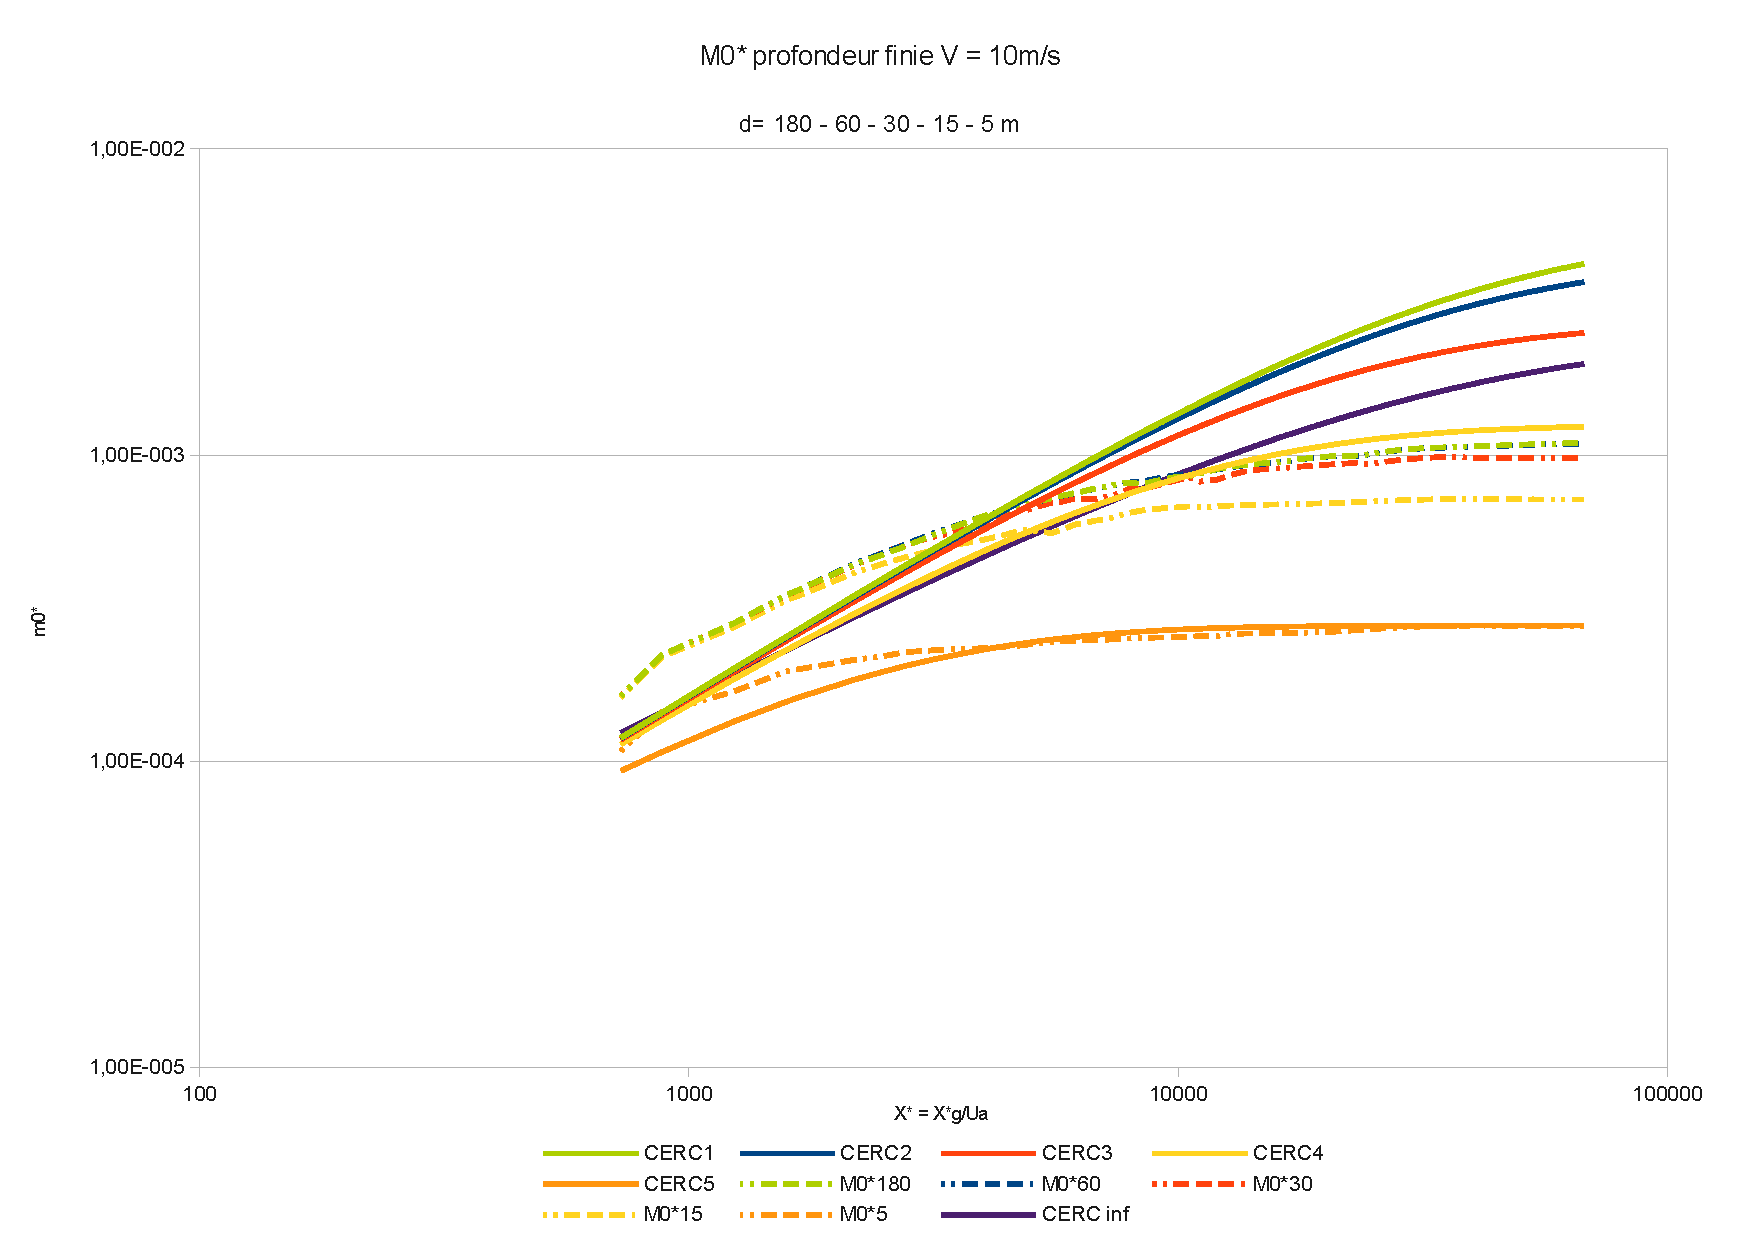
\includegraphics[scale=0.4]{m0_test7v10.pdf}\\
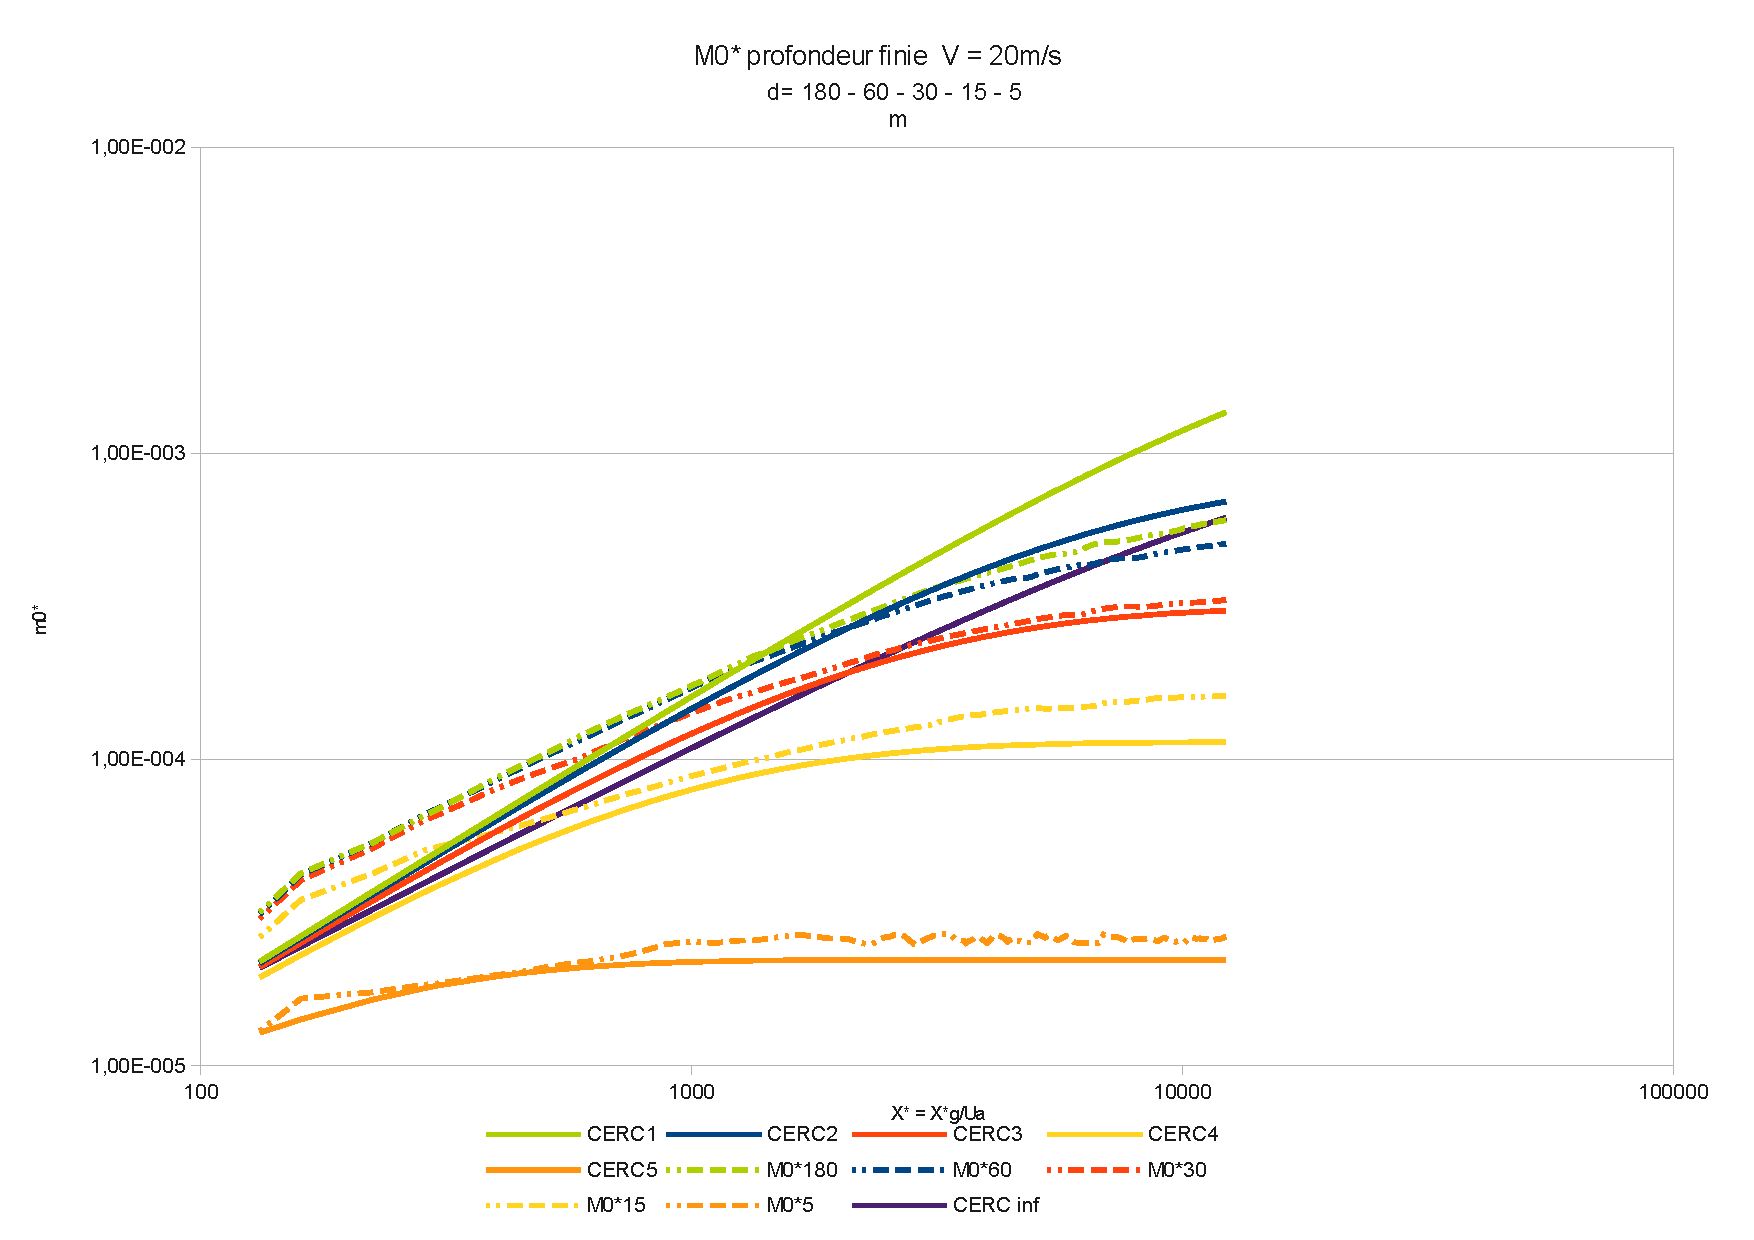
\includegraphics[scale=0.4]{m0_test7v20.pdf}\\
\caption{Comparaison of normalized Variance M0* for U10 = 10m/s (high) and 20m/s (bottom) for different depths : 5, 15, 30, 60, 180 m}
\end{figure}
Generally, TOMAWAC gives correct results if you adapt the model at the good application model. 
\section{Conclusion}
\subsection*{Infinite Depth}
This benchmark allows to verify that TOMAWAC results for simultaneous processing of different source terms are correct. A comparison with empirical formulas validates this simulation with generally matching results. The use of the exact GQM quadruplet transfers model allows the visualization of overshoots, but,CPU time are increased, so it is not advisable to use this model for big industrial cases.
\subsection*{Finite depth}
Even if a 1000 km fetch with only 5 m depth is hard to study in reality, TOMAWAC results get close to the empirical formula. Bottom friction effect seems to be well represented.
\section*{Rerences}
\bibliography{b}
ALVES J.H.G.M., BANNER M.L. (2003) : Revisiting the Pierson-Moskowitz Asymptotic Limits for Fully Developed Wind Waves. Journal of Physical Oceanography, volume 33, pp 1301 - 1323\\
 BATTJES J.A., JANSSEN J.P.F.M. (1978): Energy loss and set-up due to breaking of random waves. Proc.
16th Int. Conf. on Coastal Eng., pp 569-587.
 M. BENOIT (1996) : Fiche cas-test : G\'en\'eration d'\'etats de mer en fonction de la distance d'action du vent (fetch) \textit{Extrait de la note HE-42/96/010/B. Logiciel TOMAWAC de mod\'elisation des \'etats de mer en \'el\'ements finis, Dossier de validation de la version 1.0} \\
 CERC (1977), Shore Protection Manual. Coastal Engineering Research Center (CERC),USACE, Vicksburg, MS.\\
 CERC (1984), Shore Protection Manual. Volume 1. Coastal Engineering Research Center (CERC),USACE, Vicksburg, MS.\\
GAGNAIRE-RENOU E., BENOIT M., FORGET PH. (2010): Ocean wave spectrum properties as derived
from quasi-exact computations of nonlinear wave-wave interactions. J. Geophys. Res. C (Oceans),
Vol. 115, C12, C12058, doi:10.1029/2009JC005665\\
 HASSELMANN, K., and al., Measurements of wind-wave growth and swell decay during the Joint North Sea Wave Project (JONSWAP), Dtsh. Hydrogh. Z., Suppl. A, 8, 12, 95 pp.\\
HASSELMANN S., HASSELMANN K. (1985): Computations and parameterizations of the nonlinear energy
transfer in gravity-wave spectrum. Part I: a new method for efficient computations of the exact nonlinear
transfer integral. J. Phys. Oceanogr., vol. 15, pp 1369-1377.\\
HASSELMANN S., HASSELMANN K., ALLENDER J.H., BARNETT T.P. (1985): Computations and
parameterizations of the nonlinear energy transfer in gravity-wave spectrum. Part II: Parameterizations of
the nonlinear energy transfer for application in wave models. J. Phys. Oceanogr., vol. 15, pp 1378-1391.\\
 JANSSEN P.A.E.M. (1989): Wave-induced stress and the drag of air flow over sea waves. J. Phys.
Oceanogr., vol. 19, pp 745-754.\\
JANSSEN P.A.E.M. (1991): Quasi-linear theory of wind-wave generation applied to wave forecasting. J.
Phys. Oceanogr., vol. 21, pp 1631-1642.\\
 K.K. KAHMA \& C J. CALKOEN (1992), Reconciling discrepancies in the observed growth of
wind-generated waves. J. Phys. Oceanogr., vol. 22, pp. 1389-1405\\
 KOMEN G.J., HASSELMANN S., HASSELMANN K. (1984): On the existence of a fully developed wind-sea
spectrum. J. Phys. Oceanogr., vol. 14, pp 1271-1285.\\
KOMEN G.J., CAVALERI L., DONELAN M., HASSELMANN K., HASSELMANN S., JANSSEN P.A.E.M.
(1994): Dynamics and Modelling of ocean waves. Cambridge University Press, 1994,532 p.\\
SNYDER. R.L., DOBSON F.W., ELLIOT J.A., LONG R.B. (1981): Array measurements of atmospheric
pressure fluctuations above surface gravity waves. J. Fluid Mech., vol. 102, pp 1-59.\\ 
Van der WESTHUYSEN A. J., ZIJLEMA M., BATTJES J.A. (2007): Nonlinear saturation-based
whitecapping dissipation in swan for deep and shallow water. Coastal Eng., 54, 151-170.\\
 B W. WILSON (1965), Numerical prediction of ocean waves in the North Atlantic for
December 1959. Deutsche Hydrographische Zeitschrift, vol. 18 (3), pp. 114-130\\
YAN L. (1987): An improved wind input source term for third generation ocean wave modelling. Tech. Rep.
8, Royal Dutch Meteor. Inst.\\
I R YOUNG \& L A. VERHAGEN 1996, The growth of fetch-limited waves in water of finite
depth. Part I: total energy and peak frequency. Coastal Engg. vol. 28, pp. 47-78.\\

 








 
\end{document}
